\documentclass{mcmthesis}
\mcmsetup{CTeX = false,   % 使用 CTeX 套装时,设置为 true
		tcn = 2002121, 
		problem = E,
        sheet = true, titleinsheet = true, keywordsinsheet = true,
        titlepage = true}
\usepackage{palatino}
\usepackage{mwe}
\usepackage{graphicx}
\usepackage{subcaption}
\usepackage{float}
\usepackage{multirow}
\usepackage{indentfirst}
\usepackage{gensymb}
\usepackage[ruled,lined,commentsnumbered]{algorithm2e}
\usepackage{geometry}
\usepackage{listings}
\usepackage{fontspec}
\usepackage{booktabs}
\usepackage{amsmath}
\usepackage{color}
\usepackage{framed}
\usepackage{xcolor}
\usepackage{fontspec}
\usepackage{mathrsfs}
\usepackage{fancyhdr}
\usepackage{diagbox}
%%\usepackage{indentfirst}%%作用:对齐行
\usepackage{enumitem} 
\usepackage{mathtools}
\usepackage{setspace}
\usepackage{graphicx}

\lstset{  
 	numbers=left,                % 在左侧显示行号
 	numberstyle=\tiny\color{gray},       % 设定行号格式
 	%frame=none,                             % 不显示背景边框
 	%backgroundcolor=\color[RGB]{245,245,244},% 设定背景颜色
 	keywordstyle=\color[RGB]{40,40,255},     % 设定关键字颜色
 	numberstyle=\footnotesize\color{darkgray},       
 	commentstyle=\it\color[RGB]{0,96,96},     % 设置代码注释的格式
 	basicstyle=\fontspec{Consolas},
 	stringstyle=\rmfamily\slshape\color[RGB]{128,0,0}, % 设置字符串格式
 	showstringspaces=false,            % 不显示字符串中的空格
 	language=Python,                      % 设置语言
}
\newtheorem{definition}{Definition}
\definecolor{shadecolor}{rgb}{0.95,0.95,0.95}

\begin{document}
\linespread{0.6} %%行间距
\setlength{\parskip}{0.5\baselineskip} %%段间距
\title{title}%%标题

\date{\today}
	\begin{abstract}%%abstract	  summary的部分
		%%这里还少一段关于问题的简述
		
		Nowadays, the world produces about 310 million tons of plastic waste a year. Plastic waste has severe environmental consequences and it is predicted that if our current trends continue, the oceans will be filled with more plastic than fish by 2050.

		To address this escalating environmental crisis, in this paper, we build two models with different functions so as to deliberate strategies for different tasks proposed by ICM more specifically. The first model, \textbf{CPE} Model will provide us an ideal extent plastic waste can be reduced to. The second model,\textbf{ Multi-factor Analysis Model}, will help us measure the contribution of different policies to plastic waste reduction based on the characteristics of different regions, so that we can optimize the most suitable policy options.

		First, we divide the processing degree of plastic waste into three major parts, including collected, process, and emission. Then we build the \textbf{CPE} Model, which connect the Human Behavior and Non-Human Ecosystem. To estimate the damage extent, we define $E$ as plastic waste that cause damage to ecosystem. 
		
		Next, in order to calculate the extent plastic waste can be reduced to reach an environmentally safe level, we create a \textbf{system of differential equations} based on \textit{Logistic growth model}. By using this, we calculate an ideal $E$ which meets the least environmental damage.$($Task 1$)$
		
		Then, to reach that extent, we need to set different target for various regions. So first, we refer to the \textit{AHP} Model and develop our \textbf{ Multi-factor Analysis Model}. In this Model, we choose 4 first-level indexes, and they are determined by 6 second-level indicators. In order to set precise weights of them, we further select 13 quantitative indicators carefully and they cover the fields of \textbf{Economy}, \textbf{Education}, \textbf{Environment} and \textbf{International Relations}. Second, according to World Bank Classification criteria, we classify regions into three group.
		
		Continuing the previous model, we then discuss the impact of our chosen policy on various regions and the impact on multi-trillion-dollar plastic industry under a broad policy direction.$($Task 3$)$

        To discuss the equality and corresponding deliberate strategies$($Task 4$)$
		, we define two index $e$ and $c$, which are respectively related to plastic waste emission amount and impact, to measure the equality in different regions.  



        %%这里还有我们对国家的分类。
 

		%%这里还有一个我们的以节成果的小小说明

		
	 
	   \begin{keywords}
		\textbf{Logistic growth model, AHP Model, Multi-factor Analysis}%%\textbf{}表示加粗
		
		\end{keywords}
		
	\end{abstract}

\maketitle


\tableofcontents
\newpage
%以下为正文部分

%background可以放在这里,可以先去掉1.1的部分
\section{Introduction}
Since 2000, the world has produced as much plastic as all the preceding years combined. The cheapness, versatility and reliability of plastics have led to rapid growth in demand and production this century. The world produces about 310 million tons of plastic waste a year, and that figure is growing at 3\% a year.\par
At present, only less than 10\% meets recycling standards and become recycled plastic. The rest part is commonly treated by landfill, incineration, and dumping. These treatments cause great damage to the ecosystem since it takes more than 400 years to degrade plastics naturally. What is more, burning a ton of plastic releases as much as 2.7 tons of carbon dioxide into the atmosphere. In the part of plastic waste being collected, 1/3 of the plastic waste belongs to the garbage under improper control due to the lack of control and other reasons, which also destroy the environment.

Besides those collected, there are also 11\% plastic waste goes in nature without hunman interference. This proportion turns out to be nuch higher in developing countries than in those high income countries. 

About 90\% of uncollected or mismanaged plastic waste goes directly into terrestrial ecosystems, polluting soil and freshwater bodies, with the remaining 10\% already or about to be released into the ocean. Only 1\% of the rubbish that goes into the ocean floats on the surface, as shown in figure 1. The rest is thought to have sunk below the surface.
\begin{figure}[H]
	\centering
	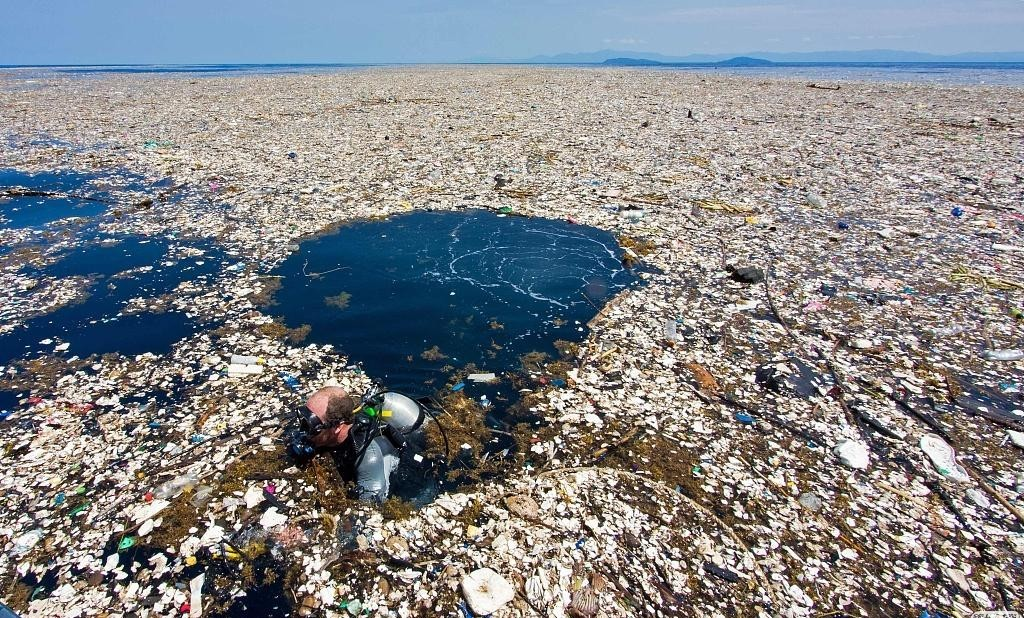
\includegraphics[width=8.59cm,height=5.18cm]{figure/introduction.png}
   \caption{plastic waste floating on water surface}
\end{figure}
In order to reduce or even further eliminate the impact of plastic waste on the environment, this paper investigates the effectiveness of a series of measures such as using plastic substitutes, issuing plastic limit policies and strengthening the supervision of plastic waste recycling through mathematical modeling, and studies the treatment of plastic waste in combination with the international situation.

		
\section{General Assumption and Nomenclature}
	 \subsection{General Assumption}
	 %%一般假设
	 \begin{itemize}     
		\item[$\blacktriangleright$]The data we collect from online databases is accurate, reliable and mutually consistent. Because our data sources are all websites of international organizations, such as World Bank and FAO, it is reasonable to assume the high quality of their data.\\
		\item[$\blacktriangleright$] In model verification, the small differences between regions in the same level that we neglect has little impact on the calculation of the weights and results.Because we divide the different regions according to the internationally recognized division basis. \\
		\item[$\blacktriangleright$] In order to better classify plastic sources and uses mentioned later in the article, we dismiss the usage time of plastic so as to equal the waste of single-use or disposable plastic product which mentioned in the problem to the waste of all types of plastic. And the latter is the same as plastic trash. We uniformly call them as plastic waste in this article.\\
		\item[$\blacktriangleright$]Besides these general assumptions, there are also other hypothesis we make for the specific models. We will present and discuss them in Section 3.\\
		\end{itemize}

  \subsection{Nomenclature}
	 %%变量定义与描述
         \begin{table}[H]
			\renewcommand\arraystretch{1.2}
			\centering
            \caption{Nomenclature}
            \begin{tabular}{cc}%%变量表
            \toprule
             Symbol&Definition\\
             \midrule
			 $E$&single-use or disposable plastic products waste emission \\
			 &that may flow into the natural environment\\
         
			 $N$&Accumulative global waste of single-use or disposable plastic products\\
			 &in the environment\\
			 
             $P_{env}$&Environmental degradation ability \\
         
			 $P_{max}$&The maximum of the environmental degradation ability\\
			 
			 $Y$&Plastic waste\\
			 
			 $Y_{NC}$&Uncollected plastic waste\\

			 $Y_{C}$&Collected plastic waste \\

			 $Y_{P}$&Collected  and managed plastic waste\\

			 $Y_{import}$&Imported plastic waste\\

			 $r_C$&Collection ratio of plastic waste \\

			 $r_P$&Processing ratio of collected and managed plastic waste\\

			 $I_S$&Index of population\\

			 $I_I$&Index of income level\\

			 $I_R$&Index of the replaceability of plastics\\

			 $I_P^Y$&Index of a policy's impact on Y\\
			 
			 $I_P^C$&Index of a policy's impact on $r_C$\\

			 $I_P^P$&Index of a policy's impact on $r_P$\\

			 $I_P^O$&Index of a policy's impact on $Y_{import}$\\

			\textbf{$W$}&Weight matrix\\

			\textbf{$I_{\textrm{i}}$}&First-level index matrix\\

			\textbf{$I_{\textrm{ii}}$}&Second-level index matrix\\

			$e$&Index used to measure the emission amount of plastic waste\\
			&in various region\\

			$c$&Index used to measure the impact of plastic waste\\
			&in various region\\

             \bottomrule
             \end{tabular}
           \end{table}
  %%section3
\section{Statement of CPE Model}
In this section, in order to estimate the maximum levels of plastic product waste that can safely be mitigated without further environmental damage, we build a model called \textbf{CPE}: \textbf{C}ollect-\textbf{P}rocess-\textbf{E}mission Model.
 
 \subsection{H part of CPE Model}
    \begin{figure}[H]
	  \centering
	  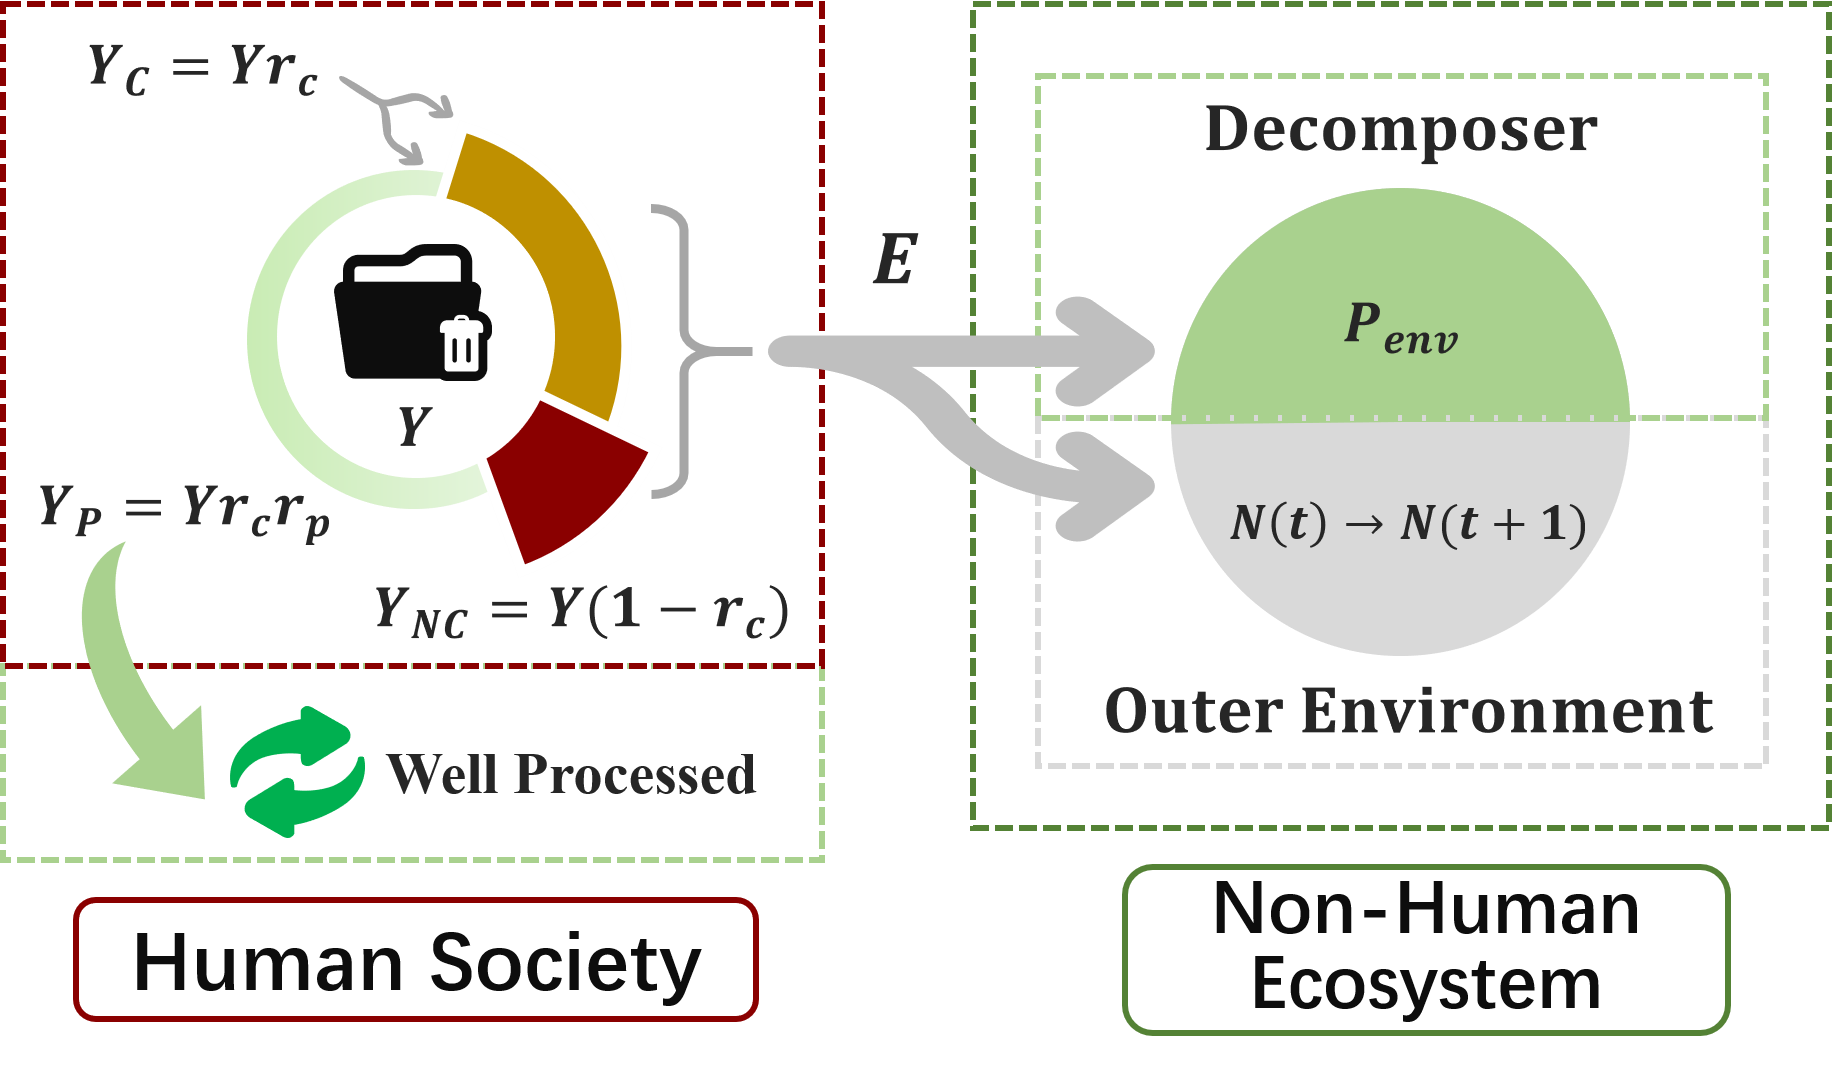
\includegraphics[width=14.65cm,height=8.42cm]{figure/CPE.png}
	  \caption{Illustration of \textbf{CPE} Model}
     \end{figure}
   
	 Based on the third hypothesis, we can assume that all disposable plastics produced will become plastic waste. In \textbf{CPE} Model, the total amount of waste produced by human society to meet the needs of production and living is recorded as $Y$. Based on the overview of the plastic products life cycle,there are two main parts in all the plastic waste $Y$. We call the plastic waste that we get from the end users through the waste collection system $Y_{C}$, and the proportion of $Y_C$ is defined as $r_C$. The rest of the totla plastic waste are not collected. They are defined as $Y_{NC}$. 
	
	The collected plastic waste $Y_C$ are further devided into managed waste and mis-managed waste. Among it, $Y_P$ reprecents managed waste, which means it goes through controlled landfilling process, or recycling, or industrial incineration. The proportion of managed waste is defined as $r_P$. On the contrary, mis-managed waste goes through open dumping or goes into uncontrolled or unspecified landfill. Mis-managed waste together with uncollected plastic waste $Y_{NC}$ are released into the natural environment without proper recycling process, making up $E$, which means $E=Y-Y_P$.
	   

 \subsection{N-H part of CPE Model and System of equations used to calculate E}
	  %%介绍计算E的方程式 
	   
	   To better this section, we make a more precise definition of variables :
	    \begin{itemize}
	      \item$E$ \qquad $E$ represents the part of plastic waste that has not been properly treated by humans or even directly discharged into the environment. It is an significant factor when we consider the level of further environmental damage caused by plastic waste.\\
	  
	      \item$N$ \qquad $N$ represents the cumulative amount of plastic waste that has been released into the environment since the invention of plastic.\\
	  
	      \item $P_{env}$ \quad $P_{env}$ is the variable we use to describe the ability of nature to degrade plastic waste. Because in the process of degrading plastic waste in nature, microorganisms make a huge contribution, we believe that this variable is related to the number of microorganisms. So we make the hypothesis that $P_{env}$ fits the \textit{Logistic growth model}. 
	    \end{itemize}

		Since we need to estimate the maximum levels of plastic product waste which meets the request from \textbf{I}nternational \textbf{C}ouncil of \textbf{P}lastic \textbf{W}aste, we need to reduce the increase of $N$. And this will depend on $E$, we will explain it in later dicussion. To reach this target, we create the systems of equations to calculate $E$.
	   
		\textbf{M}anagement, we should reduce the increase of $N$ in the \textbf{CPE} Model. 
       Here is the systems of equations we set:
	    \begin{spacing}{1.5}
	    \begin{equation}
		  \begin{cases}%%公式一
		  \frac{dN}{dt}=E-\alpha P_{env} \\
		  
		  \frac{dP_{env}}{dt}=rP_{env}(1-\frac{P_{env}}{P_{max}})\\
		  P_{max}=\lambda N-e^{\beta N}

		    \end{cases}
	     \end{equation}
		\end{spacing}
	
		The meaning of the first formula in the system of equations  $\frac{dN}{dt}=E-\alpha P_{env}$ is that: The increase in $N$ in that year is equal to $E$ in that year minus the amount of plastic waste that the natural environment can handle.
	   
		The second formula $\frac{dP_{env}}{dt}=rP_{env}(1-\frac{P_{env}}{P_{max}})$ is based on the \textit{Logistic growth model}. 

		We consider that when $N$ is less than a threshold, $P_{max}$ is positively correlated with $N$. After $N$ reaches this threshold, $P_{max}$ will decrease rapidly with the increase of $N$, which is also consistent with the law of nature: when the environment is terrible, the amount of these microorganisms will decrease sharply due to the environmental toxic effects. So we use the third formula $P_{max}=\lambda N-e^{\beta N}$ to describe this relationship. And due to the existence of obstacle factors in practice, such as human intervention activities, we will not consider the case where $P_{max}$ becomes a negative number.
	 
	
 \subsection{Answer to Task 1}
	 In order to avoid further environmental damage, which means $N$ remains at a certain level or gradully goes down, we can get a maximum value of $E$ by solving the differential equations. We set the x-coordinate zero of the \textbf{CPE} Model to the current time. So the initial values of parameters are exactly the parameters values at current moment (2019), which can be seen in Table 2. It is worth noticing that the value of $\alpha$, $\beta$, and $\lambda$ are choosen from several groups of values that are set by debugging the \textbf{CPE} Model. %初值数据来源与WWF报告
	 \begin{table}[H]
	  \renewcommand\arraystretch{1.2}
	  \centering
	 \caption{inital values of parameters used in calculating the safe $E$}
	 \begin{tabular}{|c|c|}%%initial values
        \hline
        Symbol&value\\
        \hline
		$N$&4977$\times$ 10$^6$ (ton)\\
		\hline
        $E$&115$\times$ 10$^6$ (ton)\\
		\hline
		$P_{env}$&500\\
		\hline
		$\alpha$&0.13\\
		\hline
		$r$&1000\\
		\hline
		$\beta$&3$\times$10$^{-4}$\\
		\hline
		$\lambda$&0.15\\
        \hline
        \end{tabular}
    \end{table}
	  
	 When the value of $E$ equals 95 million tons to 98 million tons, $N$ approximately keeps the current level. While having other values larger than 98 million tons, the $N$-$t$ curve keeps going up, as shown in Figure 3.
	 
      \begin{figure}[H]
		\centering
		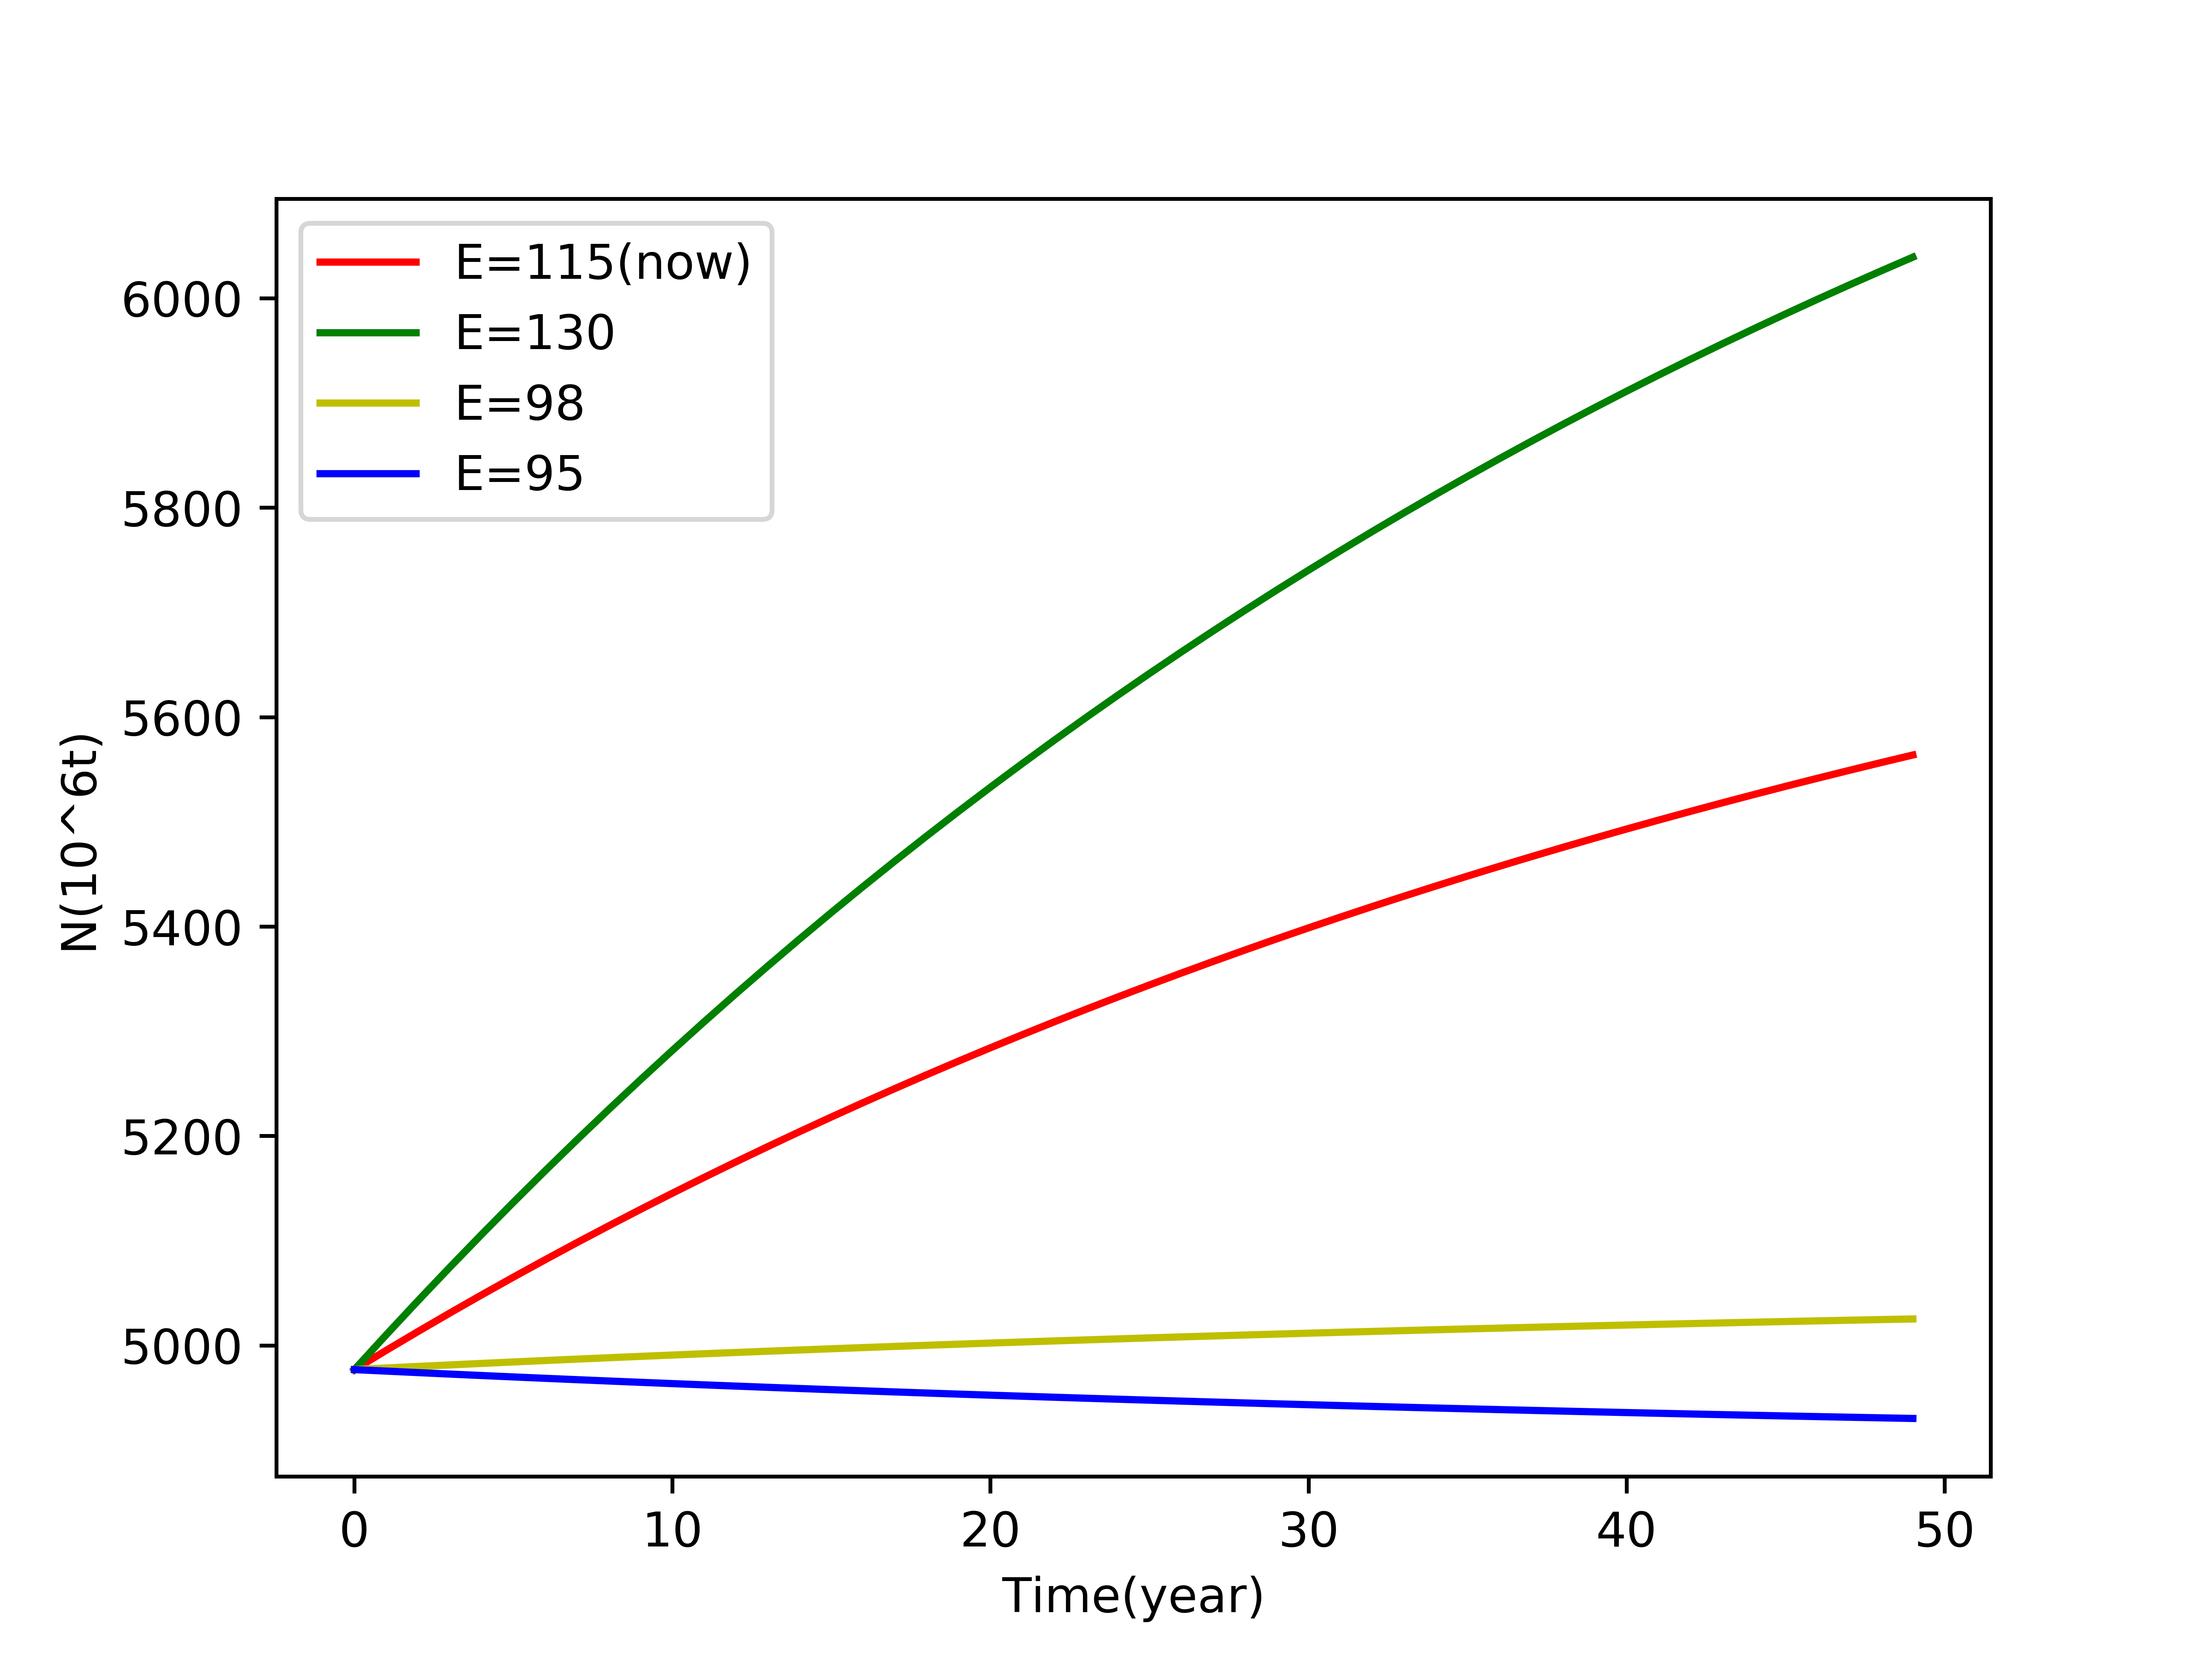
\includegraphics[width=0.8\textwidth]{figure/Estimation_of_minimal_achievable_level_plastic.png}
		 \caption{Influence of different initial $E$}
	   \end{figure}

    %文献 111\cite{Proakis2008DigitalSP}


\section{Multi-factor Analysis Model Based on AHP}
 \subsection{Statement of Multi-factor Analysis Model}
	
  \subsubsection{First-level and Second-level Indexes}
    To reduce $E$ to an environmental safe level, we have to consider many related factors that can influence $Y$, $r_C$, and $r_P$. These factors include market demand for plastic products, regional development level and per capita income, substitutability of plastics and policy. Different policies affect different aspects in this model, so we generally divide policies into 3 main categories. Policies that mainly change the market demand for disposable plastic, policies that mainly change collected rate $r_C$, and policies that change properly processed rate $r_P$. Specific analysis will be demonstrated in the following. 
	
    Given various factors above to be taken into consideration, we choose \textit{Analytic Hierarchy Process (AHP)} to help to clarify the analyzing process.
\begin{spacing}{1.4}
\begin{equation}
 \begin{bmatrix}
   
   w_{11}&w_{12}&\cdots&w_{17}\\
   w_{21}&w_{22}&\cdots&w_{27}\\
   w_{31}&w_{32}&\cdots&w_{37}\\
   w_{41}&w_{42}&\cdots&w_{47}\\
 
  \end{bmatrix}
  \textcolor{white}{\cdot}
  \begin{bmatrix}
   I_{hS}&I_{mS}&I_{lS}\\
   I_{hI}&I_{mI}&I_{lI}\\
   I_{hR}&I_{mR}&I_{lR}\\
   I_{hP}^Y&I_{mP}^Y&I_{lP}^Y\\
   I_{hP}^C&I_{mP}^C&I_{lP}^C\\
   I_{hP}^P&I_{mP}^P&I_{lP}^P\\
   I_{hP}^O&I_{mP}^O&I_{lP}^O
  \end{bmatrix}
  =
  \begin{bmatrix}
	 Y_h&Y_m&Y_l\\
	 Y_{h\ import}&Y_{m\ import}&Y_{l\ import}\\
	 r_{hC}&r_{mC}&r_{lC}\\
	 r_{hP}&r_{mP}&r_{lP}
  \end{bmatrix}
  \end{equation}
   \end{spacing}
   \begin{spacing}{0}
  
     \qquad \qquad \qquad \quad \textbf{${W}$}\qquad \qquad \qquad \quad \quad \textbf{$I_{\textrm{ii}}$}\qquad \qquad \qquad \qquad \qquad \quad \textbf{$I_{\textrm{i}}$}
   \end{spacing}

 
   \hspace*{\fill} 
	  
   The definitions of second-level indexes appeared in the matrix \textbf{$I_{\textrm{ii}}$} are as follows.
   \begin{itemize}
		\item$I_S$
			Since plastic products provide people with great convenience, we make the hypothesis that everyone has a basic need for plastic products. And considering some special regions with large population, such as India and China, their first-level indicators are   greatly affected by the population index, so we choose this second-level index $I_S$.
		\item$I_I$ 
	 
		\begin{figure} [H]
			\begin{minipage}[t]{0.5\linewidth} 
			\centering 
			\includegraphics[width=6.26cm,height=4.15cm]{Income_impact.png} 
			\caption{Share of plastic waste generated\\and uncollected by income group} 
			\label{frame} 
			\end{minipage}% 
			\begin{minipage}[t]{0.5\linewidth} 
			\centering 
			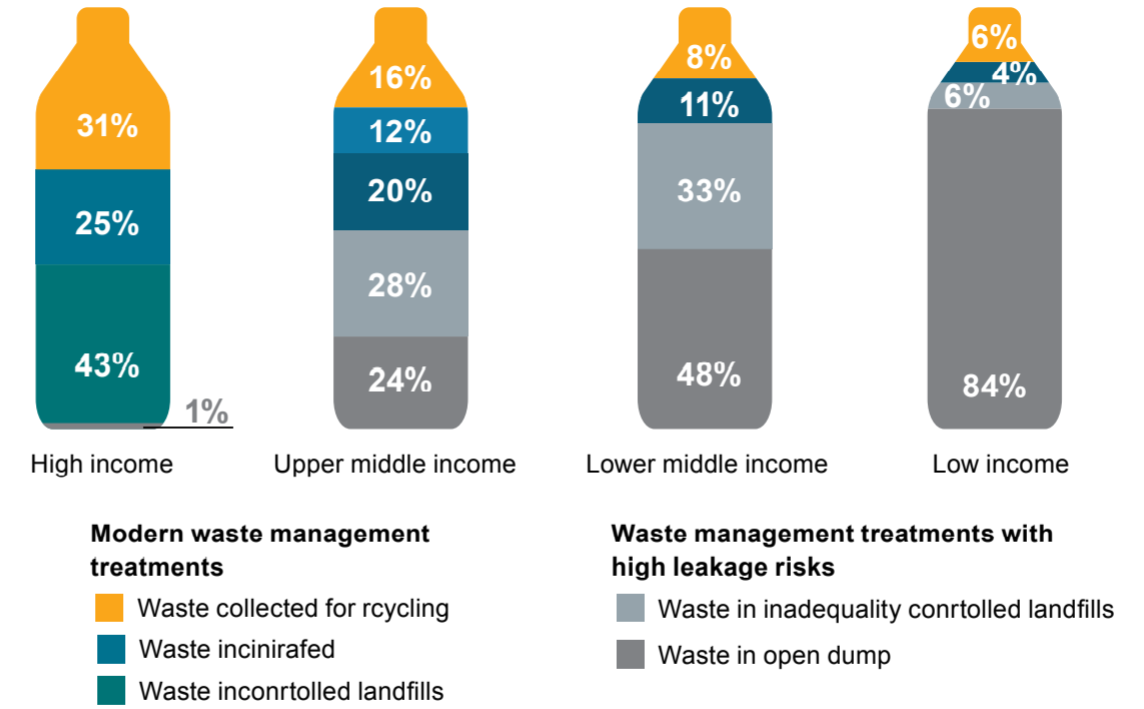
\includegraphics[width=6.66cm,height=4.39cm]{Income_and_Process.png} 
			\caption{Share of plastic waste treatment by income group} 
			\label{label} 
			\end{minipage} 
		\end{figure}


	   \begin{spacing}{0.5}
	   \hspace*{\fill}
	   \end{spacing}
	   According to the data from \textbf{WWF} $($Figure 4 and Figure 5$)$, it is obvious to find that different income levels have a great relevance to the production volume, collection rate and treatment rate of plastic waste. In order to better estimate these first-level index, we introduce this index.
		 

		\item$I_R$

		We classify plastic waste into 7 categories (PET, HDPE, PVC, LDPE, PP, PS and others) according to the classification standards established by the \textbf{P}lastics \textbf{I}ndustry \textbf{A}ssociation. In order to calculate $I_R$:
	 \begin{itemize}
	   
	   \item \textbf{Step 1}\quad We express $Y$ as $Y=\{ Y_1,Y_2,\cdots,Y_7\}$. $Y_i$ corresponds to the plastic waste of category i.
	   
	   \item \textbf{Step 2}\quad For each $Y_i$, we can estimate a corresponding fungibility $f_i$.
	   
	   \item \textbf{Step 3}\quad When we estimate $f_i$, we will consider two main indicators: technology level and difficulty of replacing this type of plastic products. After our weighted calculation processing, $f_i$ can be estimated.
	   
	   \item \textbf{Step 4}
		   \begin{equation}
			I_{R}= \sum_{i=1}^{7}f_i\left(\frac{Y_i}{Y}\right)
			 \end{equation}
			
			 \qquad Since the two indicators and the $(\frac{Y_i}{Y})$ vary between regions, it can become a second-level index by weighted calculation processing.

	   \end{itemize}
		\item{$I_P^Y$, $I_P^C$,$I_P^P$,$I_P^O$} 
		
		We list these three as part of second-level index. Not only because policies affect the first-level indexes according to various facts, but also consider that they can help us better discuss the influence caused by different policy types under regional-specific constraint.
   \end{itemize}

	
   \subsubsection{Basic frame of our Multi-factor Analysis Model}
	 In our \textbf{Multi-factor Analysis Model}, we use 4 first-level indicators, $Y$, $Y_{import}$, $r_c$ and $r_p$ to estimate $E$. Ulteriorly, 4 first-level indicators are determined by 6 second-level indicators. After nondimensionalizing second-level indicators by applying Equation (4), correspondingly we get 6 second-level indexes, $I_S$, $I_I$, $I_R$, $I_P^Y$, $I_P^C$and$I_P^P$.
	 \begin{equation}
        x_i=\frac{x_i-\bar{x}}{s}\\
	  \end{equation}
	
	  The importance of second-level indexes to first-level indexes is given by the weight matrix \textbf{${W}$}. The relationship between first-level index matrix \textbf{$I_{\textrm{i}}$} and second-level index matrix \textbf{$I_{\textrm{ii}}$} can be described by Equation (2).

	  Through \textit{AHP}, we can reduce $E$ by changing second-level indicators, since first-level indicators directly related to $E$(as shown in Equation (5)) are indicated by second-level indicators.

	  \begin{equation}
		    E=(1-r_Cr_P)(Y+Y_{import})
		\end{equation}
	
 \subsection{Answer to Task 2}
	 The indicators we consider are relatively comprehensive, and they are all indicators that can be found and estimated with accurate quantitative indicators. This makes our model highly usable. During solving task 1, we have illustrated that $E$ for current moment equals to 115. However, to reach the environmental safe standard, we need to reduce $E$ to below 98. And based on \textit{AHP} above, we can inference the change we need to make on the second-level indexes.
	 
	 Among our second-level indexes, the weight of the income level index is relatively large and it is also related to other indexes. It will affect the demand for plastic products in a country and also affect comprehensive national power, thereby influencing technology, policy and so on. So we refer to the World Bank's classification of countries to divide countries into different groups (Table 3) and analyze Task 3.
	
	 \begin{table}[H]
	  \renewcommand\arraystretch{1.6}
	  \centering
	   \caption{Our classification of regions}
	 \begin{tabular}{|c|c|}%%initial values
        \hline
        Groups&Adapted Thresholds(Per capita national income)\\
        \hline
		High-income regions&>\ \$12735\\
		\hline
        Middle-income regions&\$4126\ -\ \$12735\\
		\hline
		Low-income regions&<\ \$4126\\
        \hline
        \end{tabular}
	\end{table}
	 
	Before calculating what factors to have some change, here lists specific values for indicators, as shown in the table below. To make use of the actual number of indicators with various units, it is essential to convert them into dimensionless value, using Equation (4).

   %%大表格
   \begin{table}[H]
	\centering  
	\renewcommand\arraystretch{1.2}     
	\caption{Specific parameter value in \textit{AHP}}
	\scalebox{0.65}{
	\begin{tabular}{|c|c|c|c|ccc|c|} 
	\hline
	First-level&Second-level 
	&Quantitative Index&Units&&Actual Number&&Weight\\
	
	\cline{5-7}
	 Index&Index&&&China&European Union&India&\\
	\hline
	
	&&The total population of the area&100 million people&14.0005&5.1&13.26&0.16\\
	\cline{3-7}
	&$I_S$&Output value of plastics industry&\$100 million per year&3,274.00&6392.7&1964&0.16\\
	\cline{3-7}
	Y&&Plastic manufacturing and imports&million ton/year&118.63&145.5&70.8&0.16\\
	
	\cline{2-7}
	&$I_R$&The yield of degradable plastics&million ton/year&0.135&0.424&0.095&0.16\\
	\cline{2-7}
	&$I_I$&Per capita income&dollar/year&4044&43165&3438&0.16\\
	\cline{2-7}
	&$P_Y$&Plastic consumption reduction by the ban&100\%&24.6&50&19.8&0.33\\
	 
	\hline
	&&garbage classification Implementation rate&100\%&0.5&70&0.43&0.33\\
	\cline{3-7}
	$r_C$&$P_r^C$&Yield of recycled plastics&million ton/year&17&42&16.8&0.33\\
	\cline{3-7}
	&&Higher education proportion &100\%&14&33&12.7&0.33\\

	\hline
	&&The impact of environmental taxes&\$100 million per year&25.1&3688&10.9&0.33\\
	\cline{3-7}
	$r_P$&$P_r^P$&The impact of emission standards&100\%&22.7&50&197&0.33\\
	\cline{3-7}
	&&The size of a regulated landfill&10$^9$m$^2$&3.6262&1.7&2.42&0.33\\

	\hline
	$Y_{import}$&$P_r^O$&Garbage import volume&million ton/year&0.0516&-6.1&0.12&1\\
	\hline
	\end{tabular}}
	\end{table}
	
	In order to reduce $E$ to reach environmentally safe level, $E$ should be reduced by 17.3\% (from 115 to 95, unit million ton/year)
	
	Below are the different countries discussed separately.(In Figure 6)
     \begin{figure}[H]
		\centering
		 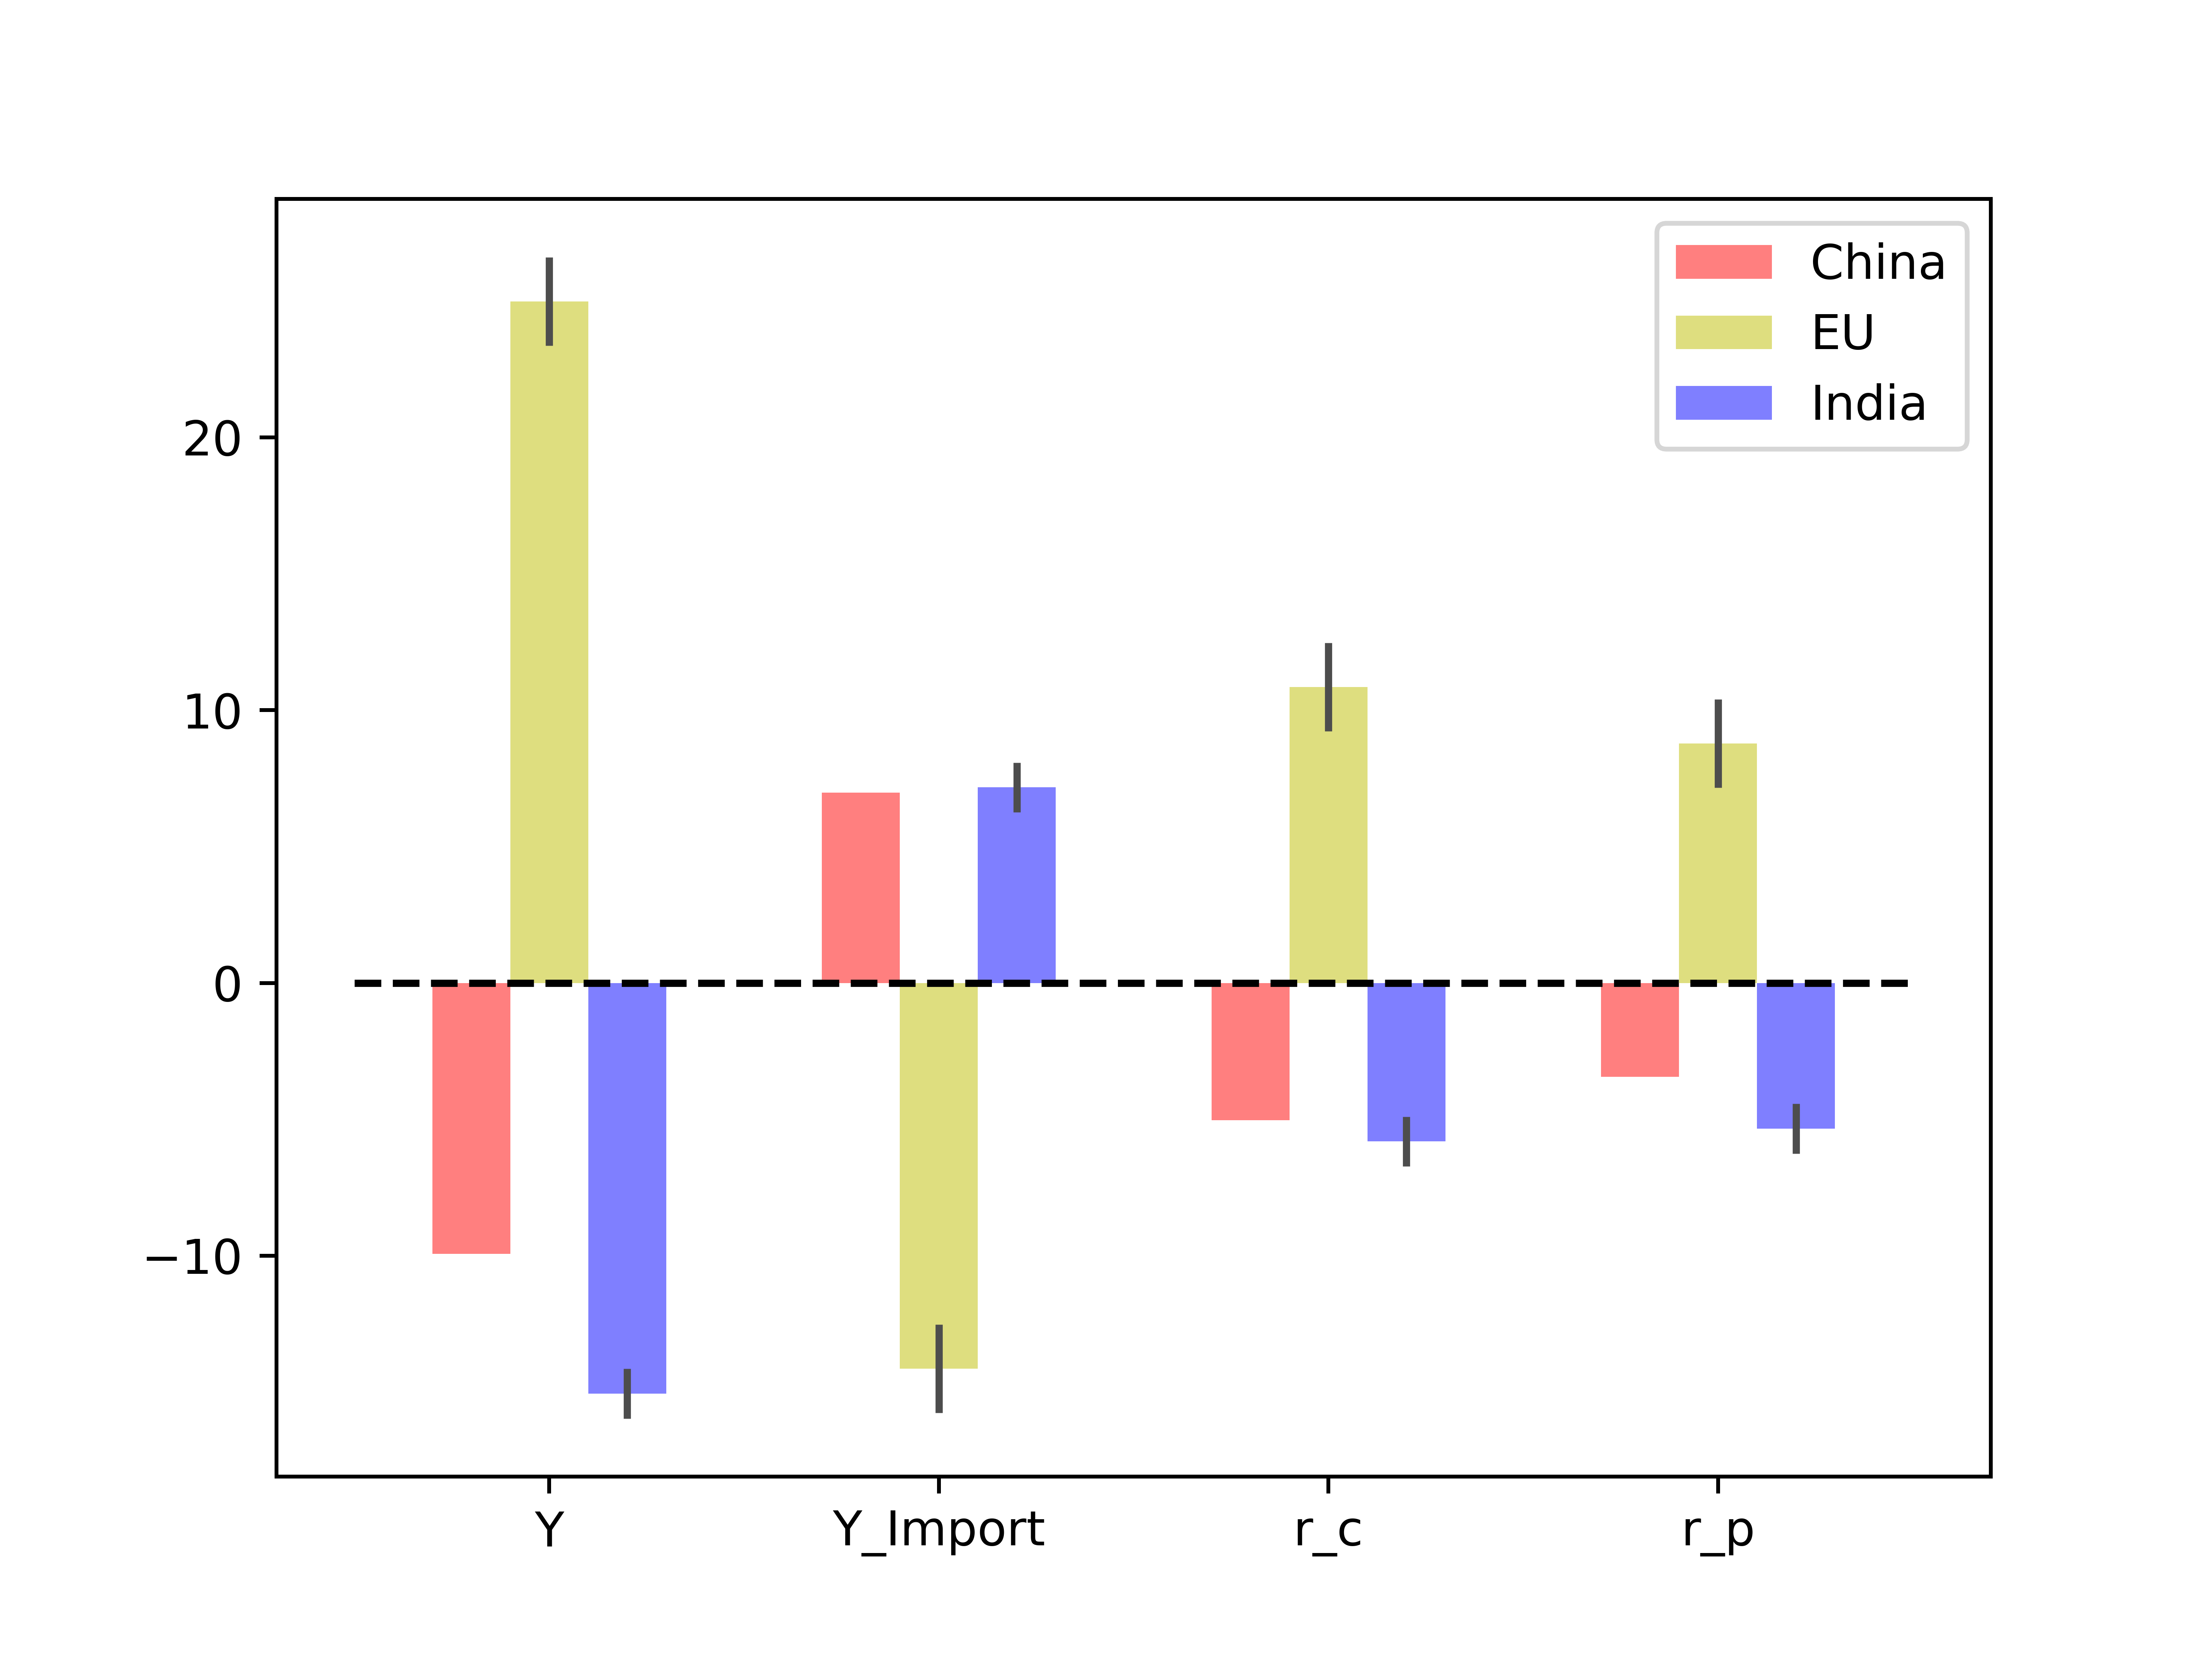
\includegraphics[width=8.98cm,height=6.39cm]{Region_Estimation.png}
		\caption{Evaluation of dimensionless first-level indexes}
	\end{figure} 

 \subsubsection{High-income regions}
	For the high income-regions like EU, their existing $r_C$ and $r_P$ levels are at a high level relatively, and there is little room for improvement. Therefore, we mainly consider making changes below to reach environmental safe standard in the high income regions. 
	\begin{itemize}
		\item Plastic production manufacturing and imports reduce from 145.5 million ton/year to 116.4 million ton/year. (declaring by 20\%)
		\item The yield of degradable plastics increase from 0.424 million ton/year to 1.06 million ton/year.(Increasing by 250\%)%The conversion rate from recycled plastics production capacity to yeild value is less than 30%.
	 \end{itemize}
	   
	 However, considering palstic export rejected by orther regions, improvement above are expected to be more significant.
	
 \subsubsection{Middle-income regions}
	 For the middle-income regions like China, their existing $Y$ is determined by population and the need for economic and technology development.The most efficient ways to reach the goal count on $r_P$ and $r_C$ increasemnt.
	 \begin{itemize}
		\item Introduce a more mandatory ban on plastics, to have 50\% reduce in plastic for disposable cutlery and pakaging.
		\item Have the implementation rate of garbage classify increase of 95\%.
		\item Introduce stricter environmental tax laws, with a 25\% increase in the tax on emissions of single-use plastic waste.
		\item Set higher standards for plastic waste processing, reducing unregulated landfill and incineration by 70\%. 
	 \end{itemize}

 \subsubsection{Low-income regions}
	 To some extent, circumstances in low income-regions are similar to middle-income regions. They both have low $r_C$ and $r_P$, due to the moral responsibility of the population, and imperfect regulations.So we omit the details for low-income regions. \par 
	 One more thing to notice is that, regions such as China and India used to import plastic waste from high-income regions. However from 2017, China has banned plastic waste import, and India has similar policies afertwards. 

	 Plastic waste import and export have aroused regional equity problem, which will be illustrated in section 6.

	

	 \section{Strategy influences}
	 In this model, we use $E$ to measure the target for the minimal achievable level of global waste of single-use or disposable plastic products. When realizing the target, $E$ is reduced from 115 Mt to 95 Mt,the strategies needed are discussed in the last section. 
	 In this section, as answer to task 3, we mainly focus on what influence those strategies are going to make.
	  \subsection{Influences on human life}
		  More than 100 countries now have bans or controls on single-use plastics or microplastics additives.\cite{EUReport}
		 In Ireland and Australia, the use of plastic bags is progressively regulated. And in Germany, India and many countries in Africa, the use of plastic bags is completely banned\cite{xanthos2017international}. There is no doubt that this will cause huge obstacles to the packaging of food and so on. Also, the restrictions on microplastics will bring many limitations to the production and use of cosmetics.
		 On the good side, if the global recycling rate  achieves  60 \%, or about 113m tonnes recycled, more than 1m new jobs could be created in the waste management and recycling system.\cite{WWFReport}
		 What is more, reducing $E$ benefits human health. Recent Eurobarometer surveys found that 74\% of European citizens are 
		 concerned about the impact on their health (74\%) and on the environment (87\%) of everyday 
		 products made of plastics.\cite{eu2018assesment}
	 \subsection{Influences on environment}
	 If no further action be taken, with an estimated 8.4 million tonnes of plastic waste entering the oceans per year \cite{jambeck2015plastic}, Within the next 15 years, 
	  the amount of plastic accumulated in the ocean between 1950 and 2015 will double. Ocean plastic pollution could reach 300 million metric tons by 2030, based on 
	 current population growth forecasts, GDP per capita 
	 projections, and current plastic waste generation per 
	 capita.\cite{WWFReport}
	 However, if all strategies takes effect, we can have marine waste gradually cleared away.
	  \subsection{Influences on the multi-trillion-dollar plastic industry}
	  Some policies requires higher taxes on plastic products and its raw materials. \textbf{On one hand}, these add to multi-trillion-dollar plastic industry‘ burden since the increasing production and management costs. \textbf{On the other hand}, these  promote the upgrading and transformation of manufacturers, increasing the reusability of plastic requires shifting supply chains from single-use to reuse business models, designing products which is safe to not only human but also the environment.  
	  Companies that take the circular economy seriously are also attractive to investors, because they are better protected from market risks related to raw materials and climate change. In Finland, for example, Business Finland, Tesi and Taaleri invest heavily in circular economy companies.\cite {Heikki2019circueco}
	 
\section{Equality}
     According to our demarcation criteria for the three regions, almost all High-income regions are located in Oceania, North America and Europe, Low-income regions are concentrated in Africa, and Middle-income regions are mostly located in Asia and South America. For the convenience of data collection and further discussion, we can match the continents to the regions we classify before. (Table 5) Due to the low number of human activities in Antarctica, it will be excluded from the discussion.
	 
	 \begin{table}[H]
		\renewcommand\arraystretch{1.6}
		\centering
		 \caption{Matches between Regions which we classify and Continents }
	   \begin{tabular}{|c|c|}%%initial values
		  \hline
		  Groups&Included continents)\\
		  \hline
		  High-income regions&Europe, North America, Oceania\\
		  \hline
		  Middle-income regions&Asia, South America\\
		  \hline
		  Low-income regions&Africa\\
		  \hline
		  \end{tabular}
	  \end{table}
  
	 
  \subsection{Current situation}
   \subsubsection{Analysis of plastic waste Emission in various regions}
	%%蓝色饼图
	\begin{figure}[H]
	 \centering
	  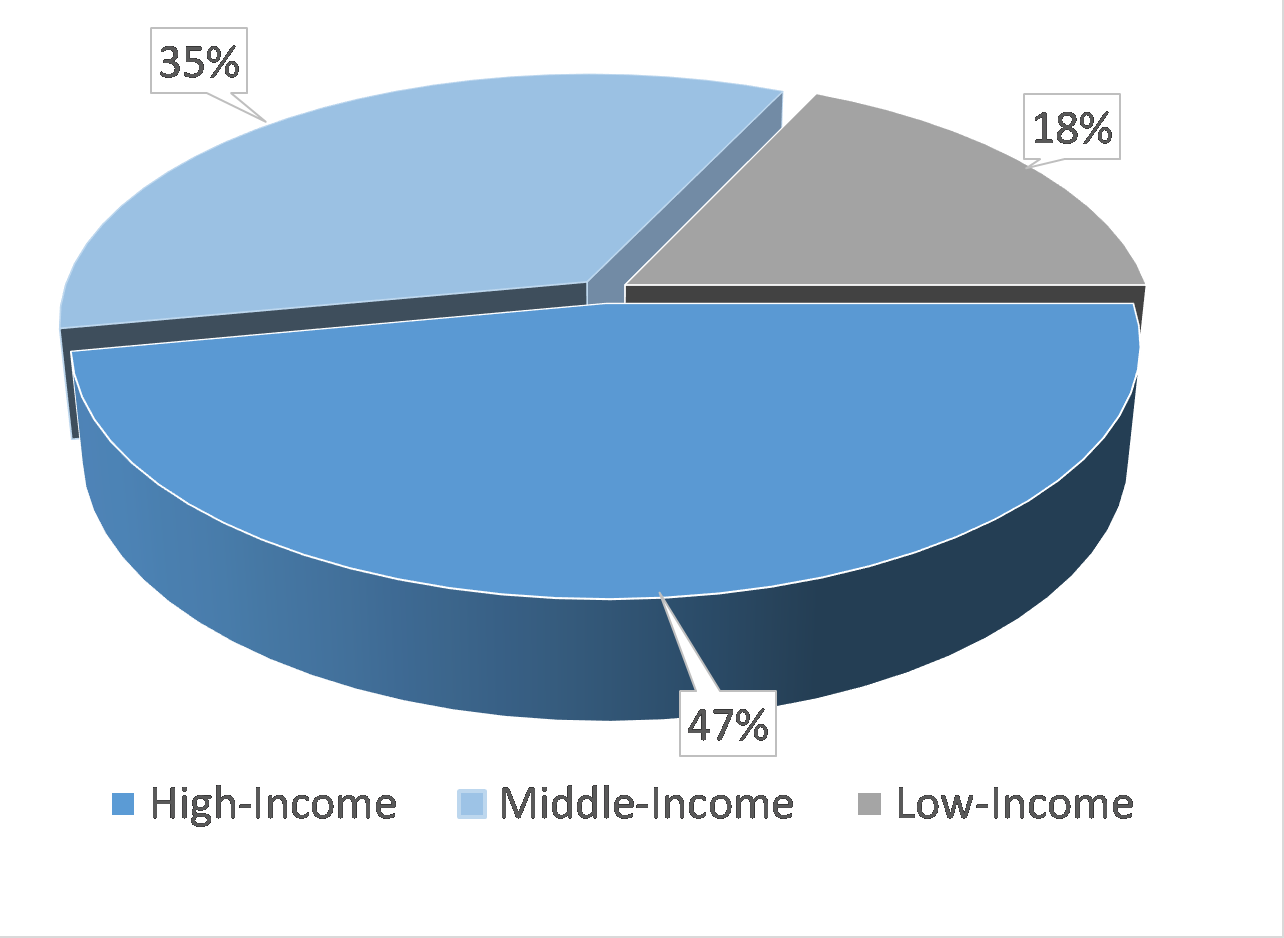
\includegraphics[width=5.74cm,height=4.31cm]{Waste_Distribution.png}
     \caption{Comparison of generating of plastic waste by regions}
	\end{figure} 
	 %%放那个绿色横向柱状图
	\begin{figure}[H]
		\centering
		 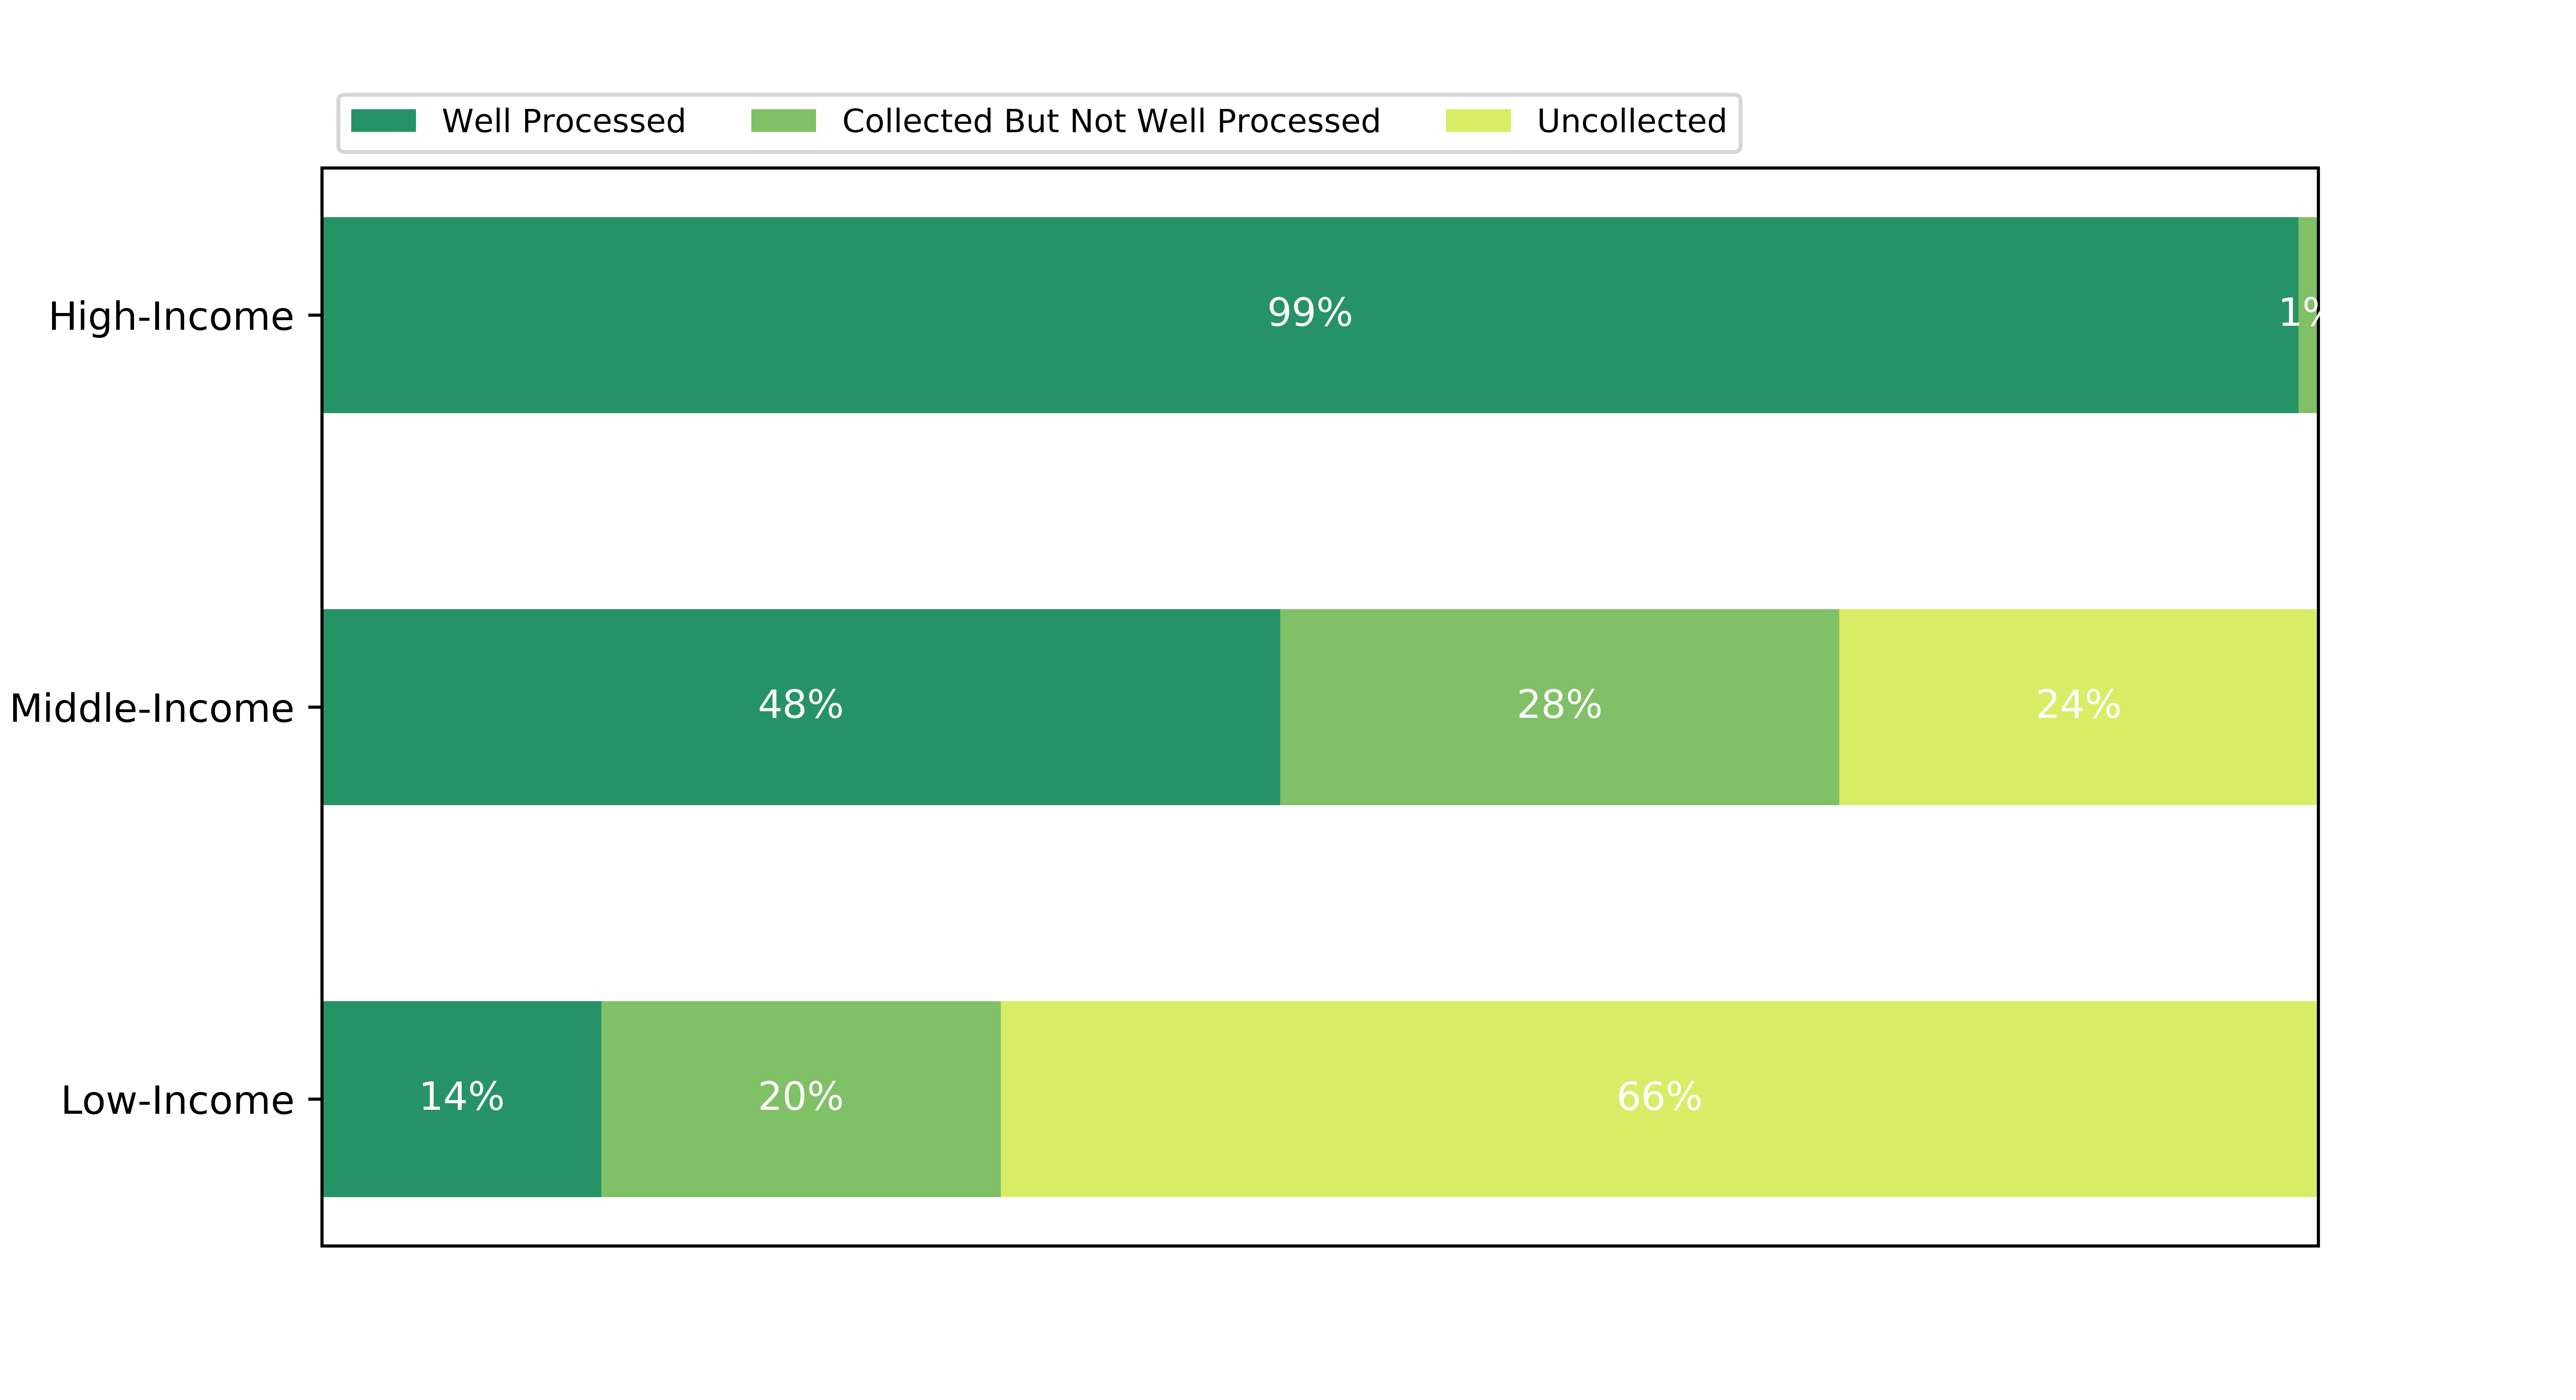
\includegraphics[width=10.93cm,height=5.94cm]{Process_Distribution.png}
		\caption{Comparison of treatment of plastic waste by regions}
	   \end{figure}
	   According to percentage of plastic waste generated by each region shown in Figure 6, together with data shown in Figure 7. We can calculate a index $e$ that reflects the amount of $E$ of each level of regions. By refering the formula $E=Y-Y_P=Y-Yr_Cr_P$, we use 
	   $e=\frac{100k_i(1-ar_Pr_C)}{\sum_{i=1}^3(100k_i(1-r_Pr_C))}$ to calculate $e$. ($k_i$ is percentage of plastic waste generated by each region) 
	   
	   A smaller $e$ represents that this region relatively produce less plastic waste emission.

	  The reslut of our calculation as follows: 
	  \begin{itemize}
       \item \quad $e$ of High-income regions:0.018
       \item \quad $e$ of Middle-income regions:0.505
       \item \quad $e$ of Low-income regions:0.477
      
	  \end{itemize}
   \subsubsection{Analysis of plastic waste Impact in various regions}
   
   We use two quantitative indicators,which are air quality and microplastic content in tap water, to assess the impact of plastic waste on various regions, which is $c$.
   \begin{table}[H]
	\centering  
	\renewcommand\arraystretch{1.2}     
	\caption{Impact of palstic waste in various regions}
	\begin{tabular}{|c|cc|cc|c|}%%initial values
		\hline
	   Regions&Air quality&Index&Microplastic  content &in tap water&$c$\\
	   \cline{2-5}
	   &Value&Weight&Value&Weight&\\
	   &$v_1$&$w_1$&$v_2$&$w_2$&\\
	   \hline
	   High-income&0.16&0.3&0.4&0.7&0.328\\
	   \hline
	   Middle-income&0.35&0.3&0.36&0.7&0.357\\
	   \hline
	   Low-income&0.49&0.3&0.24&0.7&0.315\\
	  \hline
	  \end{tabular}
	  \end{table}
	  
       
\subsection{Answer to Task 4}
 \subsubsection{Regional Differences}
   We analyze the regional equity under the global plastic pollution crisis from the perspective of regional economic development and regional import and export volume of plastic waste.

   Based on the assessment of two environmental indicators in the previous section and as shown in Figure 9, it is not difficult to see that the production of plastic waste is positively correlated with the level of economy. So, pollution is more severe in regions with higher income.
   \begin{figure}[H]
    \centering
     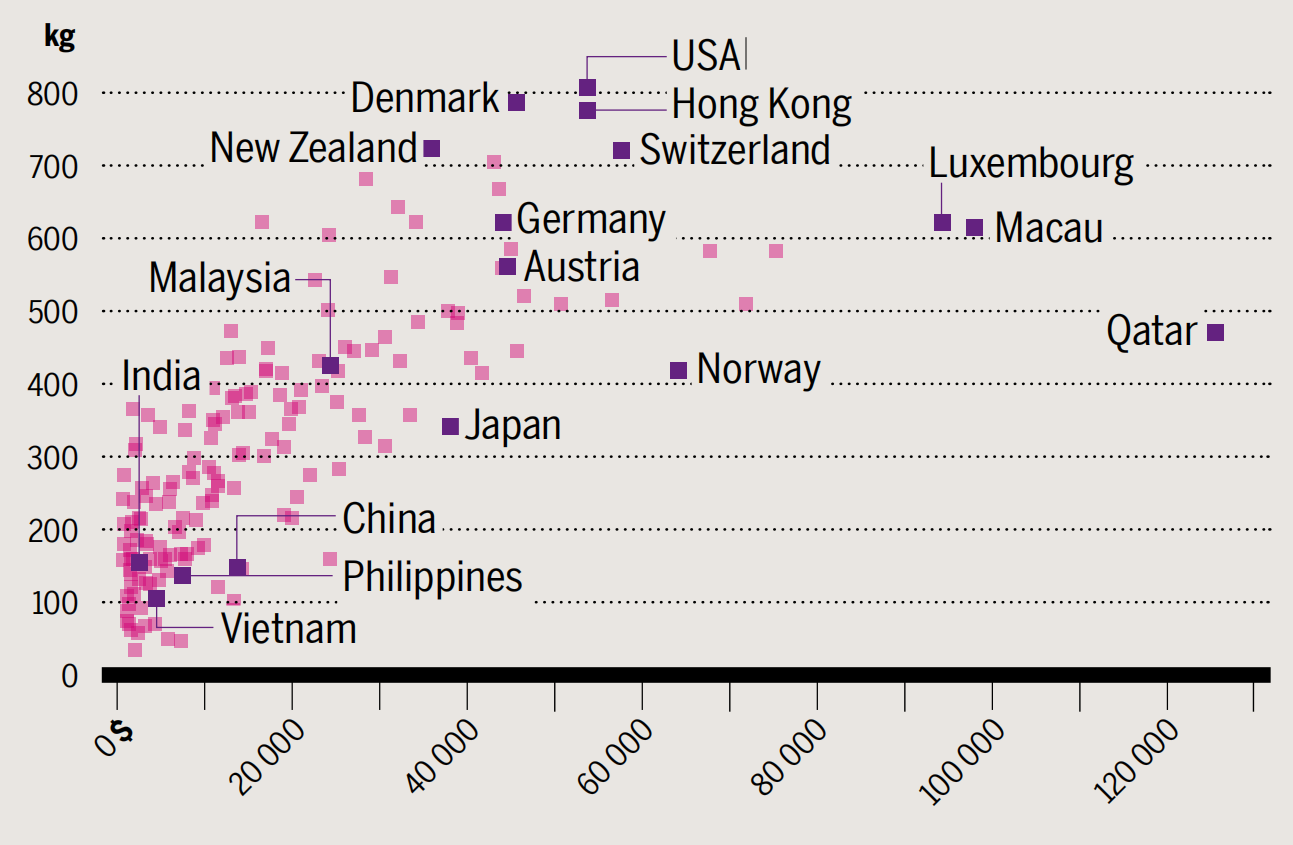
\includegraphics[width=10.93cm,height=5.94cm]{waste_income.png}
	\caption{Waste generation and gross domestic product}
   \end{figure}%source:world bank
   Though waste generated in high-income regions, they usually export large amount of waste to other countries. Nearly 50\% of waste exports are generated by G7 countries. % 引文献
   As shown in Figure 10. Worse still, middle-income regions and low-income regions have relatively poor technical level and capital of recycling, thus extremely easily to suffer from plastic pollution. Compared to waste generated locally, plastic waste import and export is more likely to trigger sensitive fairness issues.
   \begin{figure}[H]
    \centering
     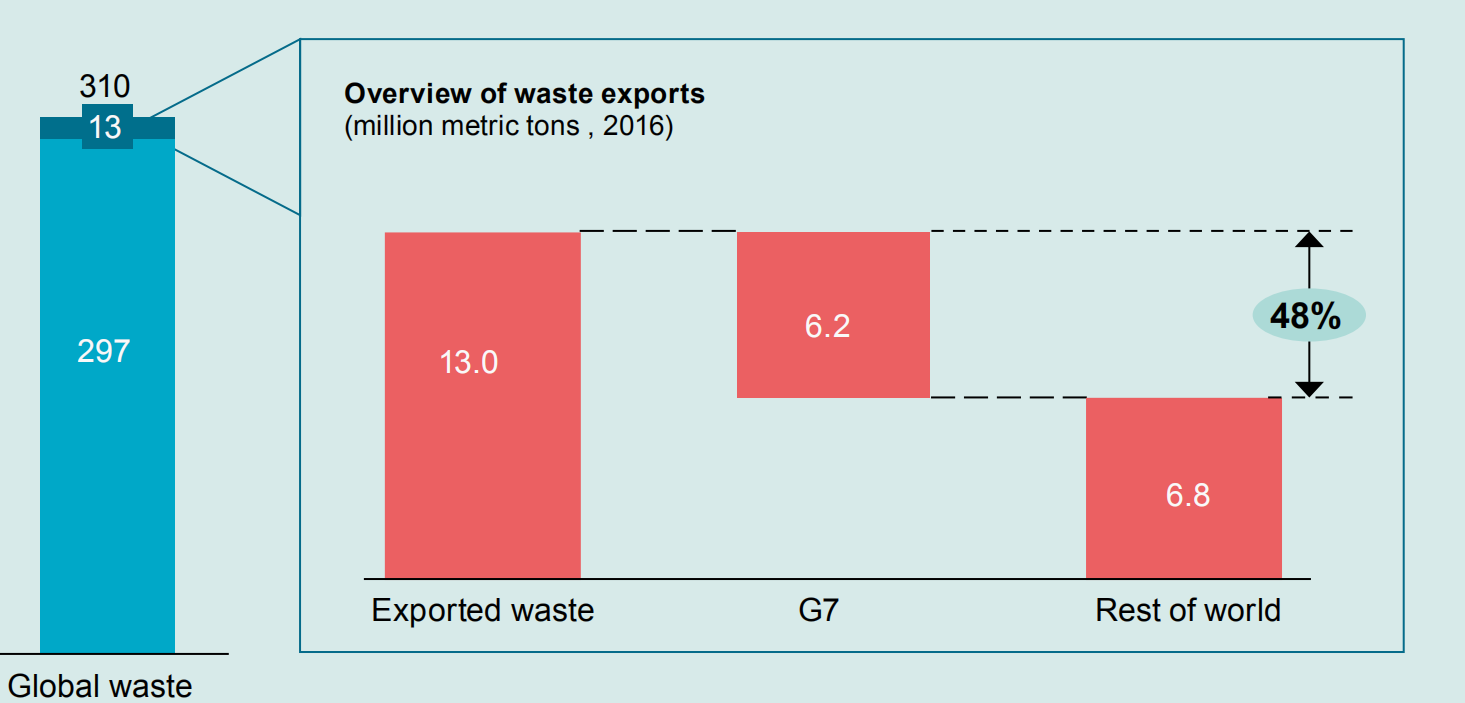
\includegraphics[width=10.93cm,height=5.94cm]{export_rate.png}
	\caption{Overiew of global waste}
   \end{figure}


 \subsubsection{Strategies}
   First of all, in order to solve the regional equity imbalance caused by plastic pollution, it is necessary to establish a unified management standard for import and export of plastic waste in the world. This helps to reduce pollution in low - and middle-income countries, and urges high-income countries to do their own plastic collection.

   For example, China introduced restrictions on imports of plastic waste, causing the country's garbage imports to plummet to 4\% of their previous level. As shown in Figure 11.
   \begin{figure}[H]
    \centering
     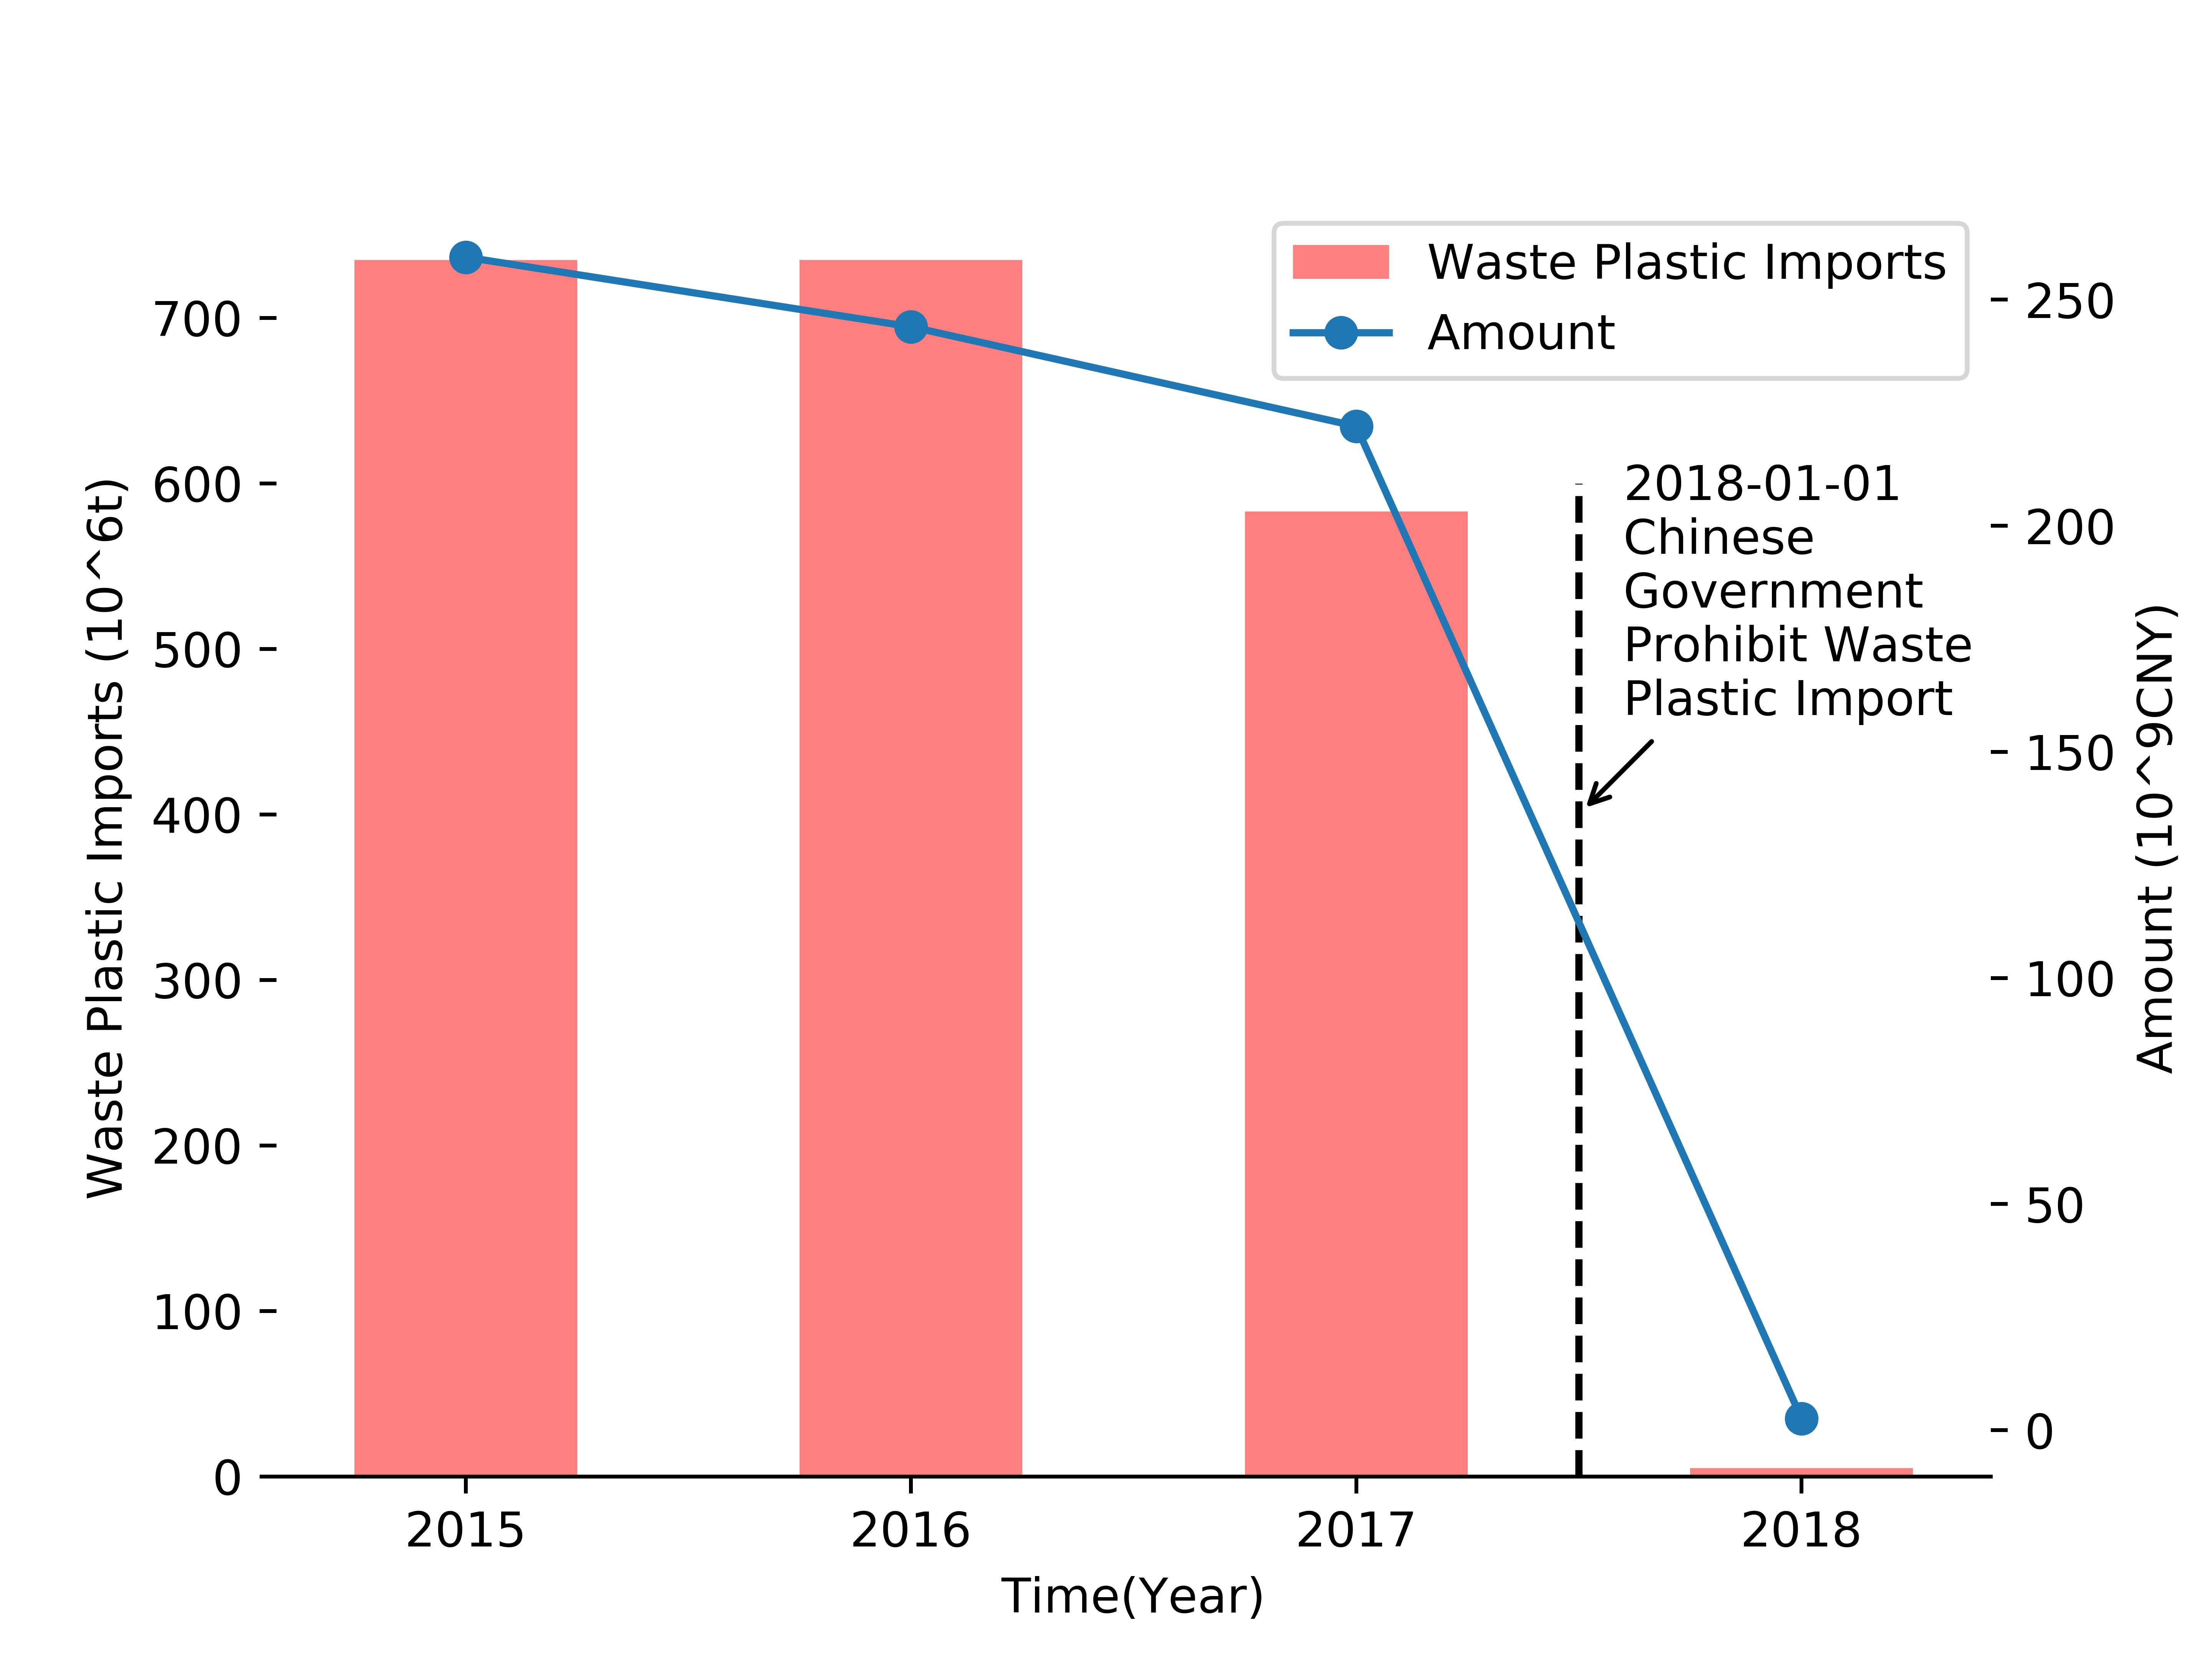
\includegraphics[width=12.93cm,height=8.94cm]{Chinese_Plastic_Import.png}
	\caption{Chinese plastic import from 2015~2018}
   \end{figure}

   In addition, to address the root of the problem and resolve this tragedy of the commons, a systems approach, deploying tactical and strategic interventions across the trade chain, is needed to create a path to no plastic in nature.
   \begin{itemize}
    \item Create global commitment through a multilateral agreement.
    \item Price plastics to reflect the natural environmental cost of the process from plastic production to waste.
    \item Promote and popularize the use of alternative materials for plastics.
    \item Help low-income countries develop efficient technologies for recycling and processing plastics.
    \item Enhance transparency and a governance system to hold every nation accountable for implementing treaty obligations.
\end{itemize}


\section{Model Analysis}
\subsection{Sensitivity Analysis}
Our CPE model contains several parameters. We determine some of the parameters through least square fitting, some of them by knowledge in the literature, and other methods. In this section,
we would like to produce a sensitivity analysis to show whether our model is sensitive to different
values of parameters,mostly on parameter $N$. 
\begin{figure}[H]
    \centering
     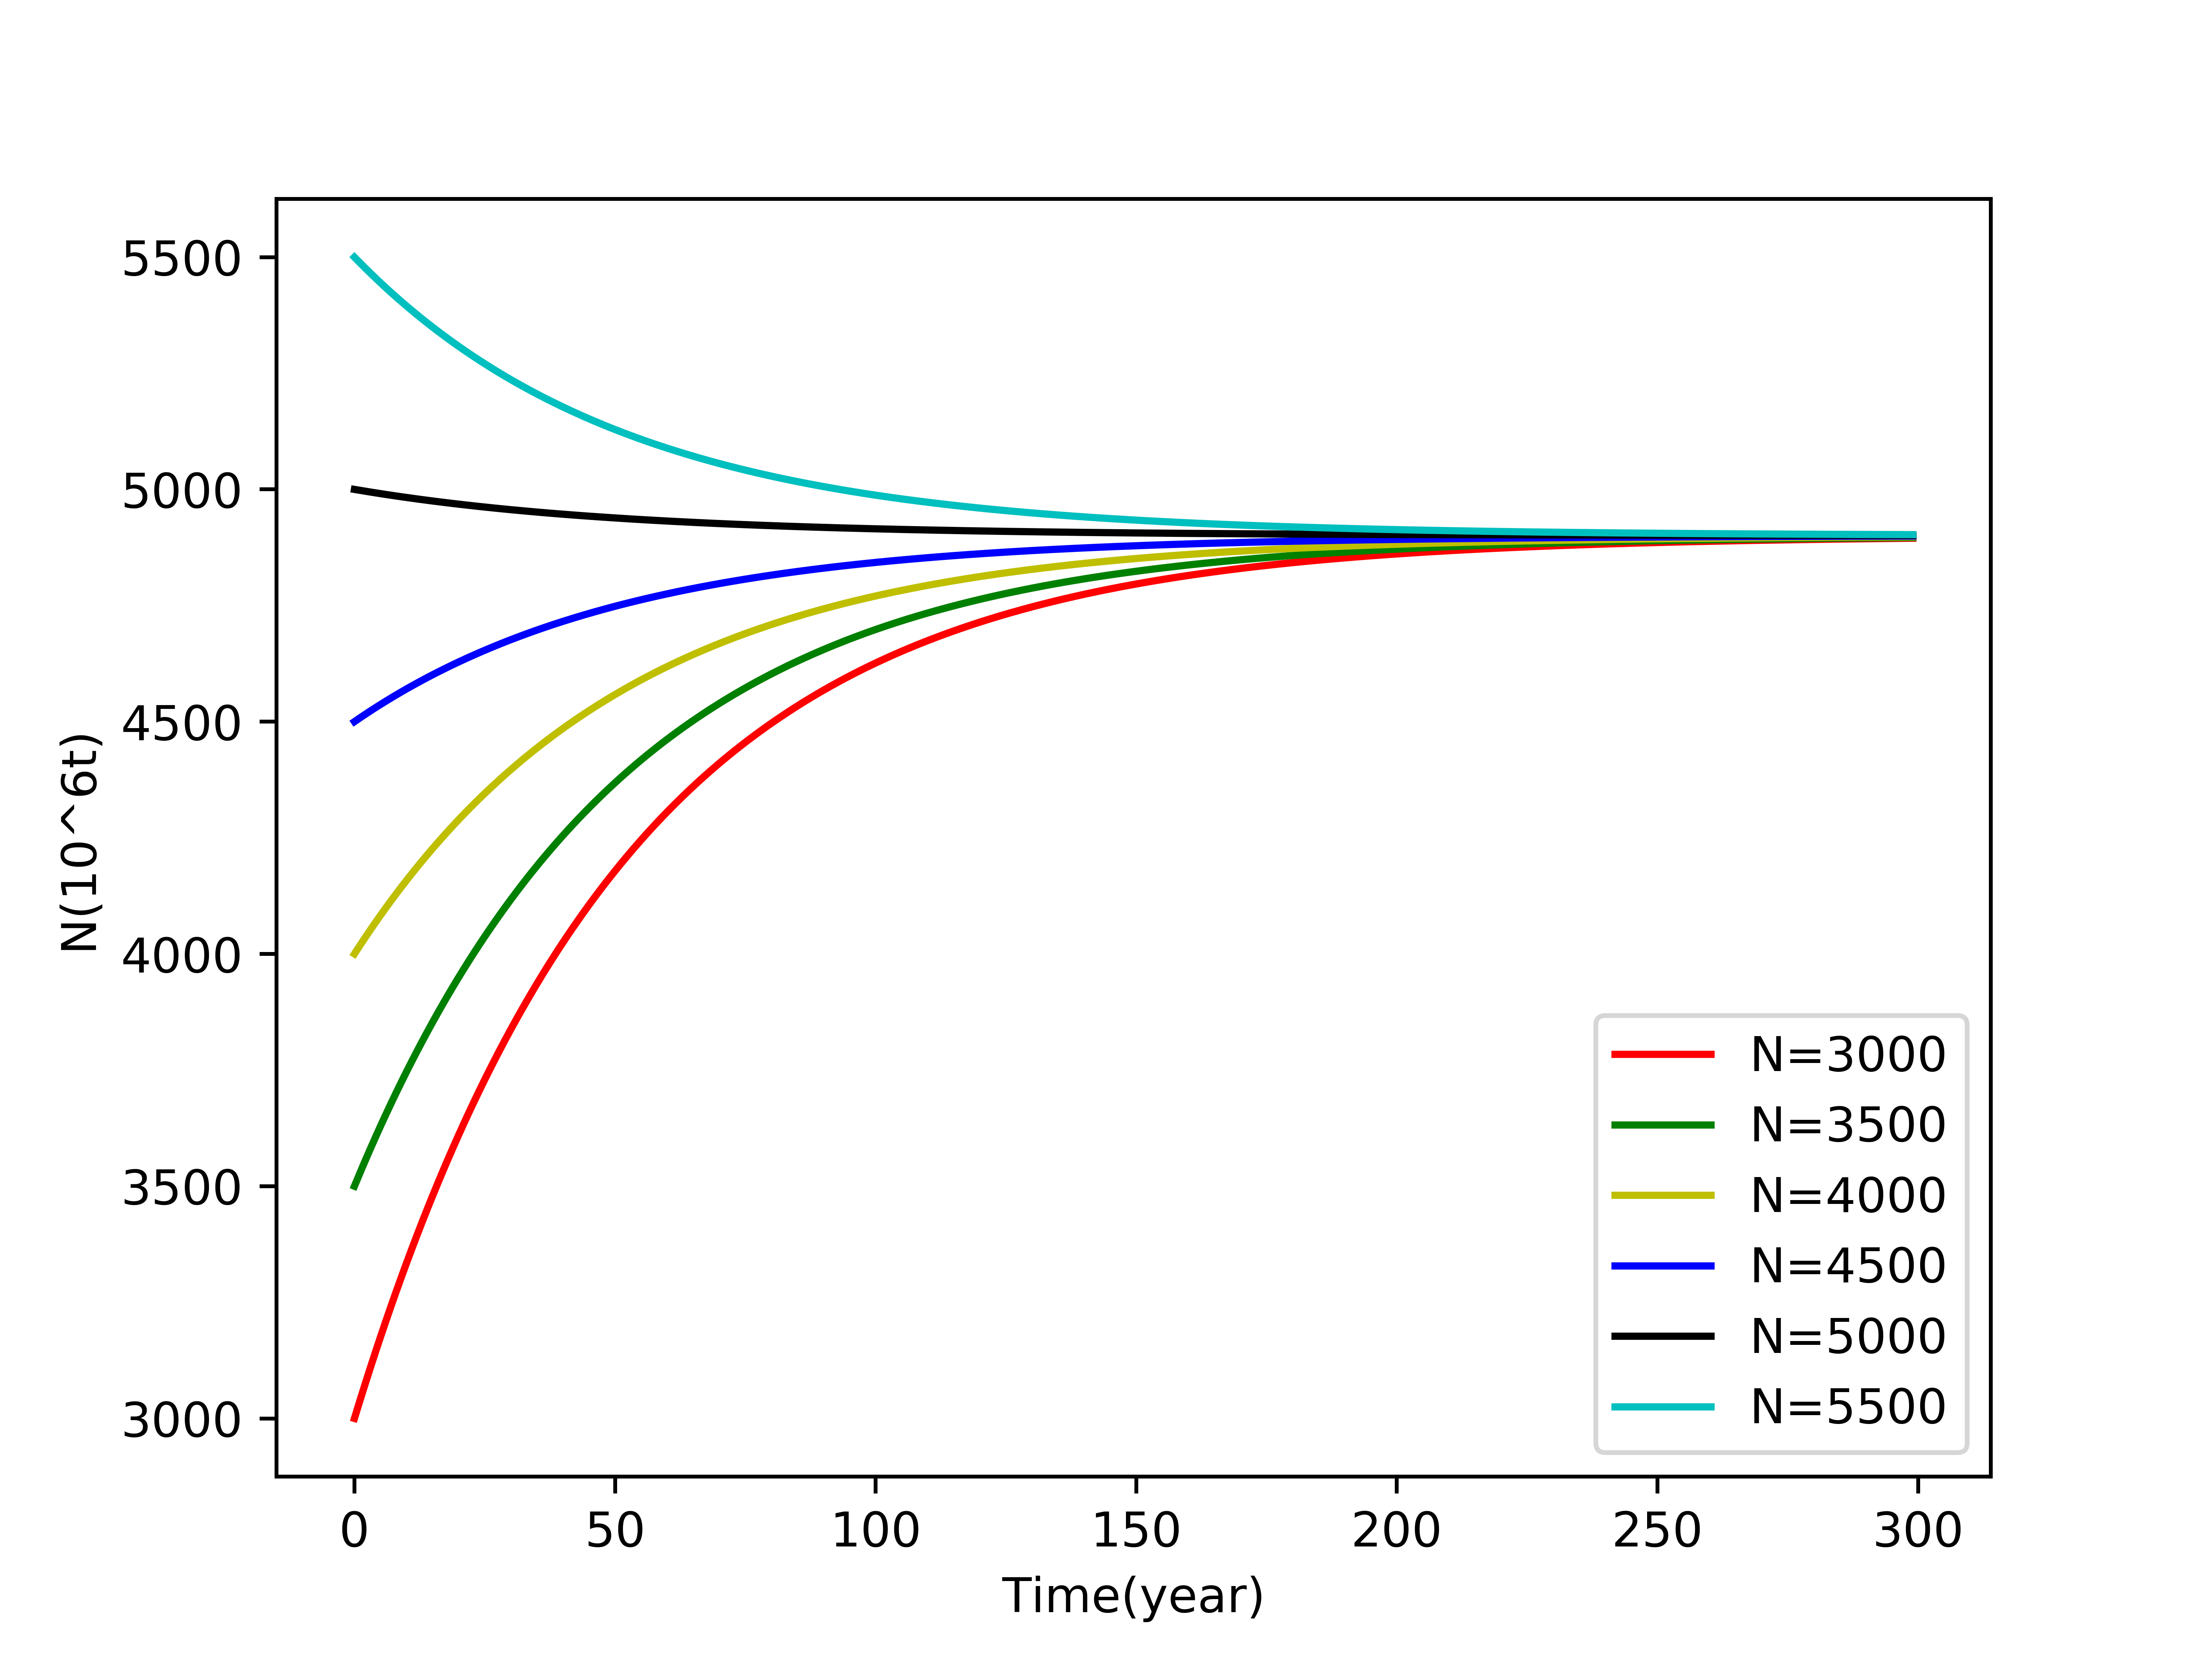
\includegraphics[width=12.93cm,height=8.94cm]{sensitivity_analysis.png}
	\caption{sensitivity analysis}
   \end{figure}

This time, $E$ is fixed to be 95(the target we expect).Other parameters are set to be the same as in Table 2.
We vary $N$ value from 3000 to 6000 by 500. Figure 12 shows that the N restrain itself to the same value ultimately. Therefore, we come to the conclusion
that our model is not sensitive to $N$. 



 \subsection{Strengths and Weaknesses}
 \subsubsection{Strengths}
	\begin{enumerate}
	 \item Various parameters in the \textbf{CPE} model accurately simulate the process of plastic production, waste collection, process and emission in real life, which has great practical significance. And in \textbf{CPE} model, the mathematical meaning of achieving the level of environmental safe standard is defined by setting $N$.
	 \item \textbf{Multi-factor Analysis Model} Based on \textit{AHP} helps to make complex thinking process as digital and hierarchical as possible. It can effectively integrate qualitative analysis and quantitative analysis, and has better properties such as substitutability, mutual capacitance and symmetry.
     \item The indicators we consider are relatively comprehensive, and they are all indicators that can be found and estimated with accurate quantitative indicators. This makes our model highly usable. \\
     \item Use accurate and frequently used data. From the very beginning of our analysis, we emphasizeon mining useful data.  Only with these dependable data, we can conclude that the model we built is appropriate.\\
     \item Use a lot of detailed tables and fancy visualization to present the statistical results of the model analysis.\\
	
	\end{enumerate}
 
\subsubsection{Weaknesses}
   \begin{enumerate}
    \item We can't always find the data related to all the countries in the Low-income region very completely. We have to replace it with the most representative country data (such as Uganda).\\
    \item By applying \textit{AHP}, we add some subjectivity to the whole model.
    \item We simplify the process of degrading plastics in nature and believe that this natural degradation ability is the same in all regions, and the actual situation is more complicated.\\
   \end{enumerate}


\section{Conclusion}
  Using \textbf{CPE} Model and \textbf{Multi-factor Analysis Model}, the target for the minimal achievable level of global 
  waste of single-use or disposable plastic products is determined by $E$ equals 95 Mt.
  Main strategies for different regions based on our model$($more specific datas are shown in other sections$)$:
  \begin{itemize}
	\item \quad For High-level regions: Based on their high-tech level, they can focus on reducing the production costs of degradable plastics to make its yield increase from 0.424 million ton/year at least to 1.06 millionton/year.$($Increasing by 250\%$)$ Take action to Mobilize the activities of local waste disposal companies to reduce the dependence on exporting plastic waste.
	\item \quad For Middle-level regions: Considering their demand of development, the restrictions on the production volume of its plastic products can be temporarily relax. We suggest that they should Set higher standards for plastic waste processing, reducing unregulated landfill andincineration by 70\%, or introduce more efficient plastic waste management methods.
	
	\item \quad For Low-level regions: The development needs of these regions are high, and due to technological constraints, they received a great impact from the pollution. However, considering that pollution enters the environment, it affects not only local residents, but also become global impact in the long run. The best way is to introduce better plastic waste treatment technology as quickly as possible.
   
	\end{itemize}
	Those strategies have significant influence on human life, environment and plastic industry.


\bibliographystyle{IEEEtran}
\bibliography{ref}

\newpage
\begin{appendices}

\section{CPE model}
\begin{lstlisting}%源代码	
	import scipy.integrate as spi
	import numpy as np
	import matplotlib.pyplot as plt
	# define time, constants and initial statess
	N1 = 4977  # initial N
	P_env = 500  # initial P_env
	E = [115, 130, 98, 95]  # E
	alpha = 0.13  # N1:amount of waste
	lamda = 0.15
	r = 1000
	beta = 3e-4
	t_range = np.arange(0, 50)
	INPUT = []
	for i in range(4):  # for each E, create input series
		INPUT.append([N1, P_env, E[i]])

	def diff_eqs(INP, t):
		y = np.zeros(3)
		v = INP
		y[0] = v[2] - alpha * v[1]
		K = lamda * v[0] - np.exp(beta * v[0])
		y[1] = r * v[1] * (1 - v[1] / K)
		y[2] = 0
		return y
	
	# run and ploting (for each different E)
	style = ['-r', '-g', '-y', '-b']
	for i in range(4):
		RES = spi.odeint(diff_eqs, INPUT[i], t_range)
		plt.plot(RES[:, 0],style[i],label="E="+str(E[i]))
	
	plt.legend(loc="best")
	# plt.title('Influence of different initial E')
	plt.xlabel('Time(year)')
	plt.ylabel('N(10^6t)')
	plt.show()
\end{lstlisting}
\newpage
\section{AHP model}
\begin{lstlisting}
	import numpy as np
	import pandas as pd
	import matplotlib.pyplot as plt
	W = np.array([
		[10, 3, 2, 5, 0, 0, 0],
		[0, 0, 0, 0, 10, 0, 0],
		[5, -1, 0, 0, 0, 3, 0],
		[5, 0, 0, 0, 0, 0, 3]
	])  # the matrix W

	# Read from excel file
	df = pd.read_excel("data/data for AHP.xlsx",
					   sheet_name="Input", index_col="Region")
	data = df.values
	
	# get result
	result = pd.DataFrame((W @ data.T).T, index=df.index,
				columns=["Y", "Y_Import", "r_c", "r_p"])
	
	# write result to excel file
	nan_excel = pd.DataFrame()
	nan_excel.to_excel("result\Region_Estimaiton_Result.xlsx")
	writer = pd.ExcelWriter("result\Result.xlsx")
	result.to_excel(writer, sheet_name="pre")

	# standardize output
	result = result.apply(lambda x: ((x-np.mean(x))/np.std(x))) 
	result.to_excel(writer, sheet_name="standard")
	writer.save()

	# draw
	result = result.T
	index = np.arange(4)
	error_config = {'ecolor': '0.3'}
	bar_width = 0.25
	fig, ax = plt.subplots()
	
	rect0 = ax.bar(index - bar_width, result["China"], bar_width, 
					color='#FFFF99', label="China")
	rect1 = ax.bar(index, result["EU"], bar_width,
					color='#FFCC99', label="EU")
	rect2 = ax.bar(index + bar_width, result["India"], bar_width,  
					color='#FF9999',label="India")
	# add axis
	ax.hlines(0, -0.5, 4, colors='k', linestyles="dashed")
	# add xticks
	for i in range(4):
		if i==0:
			plt.text(i - 0.07, -0.15, result.index[i])
		elif i==1:
			plt.text(i - 0.3, -0.15, result.index[i])
		else:
			plt.text(i - 0.1, -0.15, result.index[i])
	ax.set_xticks([])
	
	ax.legend(loc="best")
	plt.savefig("figure\Region_Estimation.png", dpi=900)
	plt.show()
	
\end{lstlisting}



\end{appendices}
\end{document}
